% Options for packages loaded elsewhere
\PassOptionsToPackage{unicode}{hyperref}
\PassOptionsToPackage{hyphens}{url}
%
\documentclass[
]{article}
\usepackage{amsmath,amssymb}
\usepackage{iftex}
\ifPDFTeX
  \usepackage[T1]{fontenc}
  \usepackage[utf8]{inputenc}
  \usepackage{textcomp} % provide euro and other symbols
\else % if luatex or xetex
  \usepackage{unicode-math} % this also loads fontspec
  \defaultfontfeatures{Scale=MatchLowercase}
  \defaultfontfeatures[\rmfamily]{Ligatures=TeX,Scale=1}
\fi
\usepackage{lmodern}
\ifPDFTeX\else
  % xetex/luatex font selection
\fi
% Use upquote if available, for straight quotes in verbatim environments
\IfFileExists{upquote.sty}{\usepackage{upquote}}{}
\IfFileExists{microtype.sty}{% use microtype if available
  \usepackage[]{microtype}
  \UseMicrotypeSet[protrusion]{basicmath} % disable protrusion for tt fonts
}{}
\makeatletter
\@ifundefined{KOMAClassName}{% if non-KOMA class
  \IfFileExists{parskip.sty}{%
    \usepackage{parskip}
  }{% else
    \setlength{\parindent}{0pt}
    \setlength{\parskip}{6pt plus 2pt minus 1pt}}
}{% if KOMA class
  \KOMAoptions{parskip=half}}
\makeatother
\usepackage{xcolor}
\usepackage[margin=1in]{geometry}
\usepackage{longtable,booktabs,array}
\usepackage{calc} % for calculating minipage widths
% Correct order of tables after \paragraph or \subparagraph
\usepackage{etoolbox}
\makeatletter
\patchcmd\longtable{\par}{\if@noskipsec\mbox{}\fi\par}{}{}
\makeatother
% Allow footnotes in longtable head/foot
\IfFileExists{footnotehyper.sty}{\usepackage{footnotehyper}}{\usepackage{footnote}}
\makesavenoteenv{longtable}
\usepackage{graphicx}
\makeatletter
\def\maxwidth{\ifdim\Gin@nat@width>\linewidth\linewidth\else\Gin@nat@width\fi}
\def\maxheight{\ifdim\Gin@nat@height>\textheight\textheight\else\Gin@nat@height\fi}
\makeatother
% Scale images if necessary, so that they will not overflow the page
% margins by default, and it is still possible to overwrite the defaults
% using explicit options in \includegraphics[width, height, ...]{}
\setkeys{Gin}{width=\maxwidth,height=\maxheight,keepaspectratio}
% Set default figure placement to htbp
\makeatletter
\def\fps@figure{htbp}
\makeatother
\setlength{\emergencystretch}{3em} % prevent overfull lines
\providecommand{\tightlist}{%
  \setlength{\itemsep}{0pt}\setlength{\parskip}{0pt}}
\setcounter{secnumdepth}{-\maxdimen} % remove section numbering
\newlength{\cslhangindent}
\setlength{\cslhangindent}{1.5em}
\newlength{\csllabelwidth}
\setlength{\csllabelwidth}{3em}
\newlength{\cslentryspacingunit} % times entry-spacing
\setlength{\cslentryspacingunit}{\parskip}
\newenvironment{CSLReferences}[2] % #1 hanging-ident, #2 entry spacing
 {% don't indent paragraphs
  \setlength{\parindent}{0pt}
  % turn on hanging indent if param 1 is 1
  \ifodd #1
  \let\oldpar\par
  \def\par{\hangindent=\cslhangindent\oldpar}
  \fi
  % set entry spacing
  \setlength{\parskip}{#2\cslentryspacingunit}
 }%
 {}
\usepackage{calc}
\newcommand{\CSLBlock}[1]{#1\hfill\break}
\newcommand{\CSLLeftMargin}[1]{\parbox[t]{\csllabelwidth}{#1}}
\newcommand{\CSLRightInline}[1]{\parbox[t]{\linewidth - \csllabelwidth}{#1}\break}
\newcommand{\CSLIndent}[1]{\hspace{\cslhangindent}#1}
\ifLuaTeX
  \usepackage{selnolig}  % disable illegal ligatures
\fi
\IfFileExists{bookmark.sty}{\usepackage{bookmark}}{\usepackage{hyperref}}
\IfFileExists{xurl.sty}{\usepackage{xurl}}{} % add URL line breaks if available
\urlstyle{same}
\hypersetup{
  pdftitle={A ciliary photoreceptor-cell circuit mediates pressure response in marine zooplankton},
  pdfkeywords={pressure sensation, plankton, sensory systems, cilia},
  hidelinks,
  pdfcreator={LaTeX via pandoc}}

\title{A ciliary photoreceptor-cell circuit mediates pressure response
in marine zooplankton}
\author{true}
\date{}

\begin{document}
\maketitle

\hypertarget{abstract}{%
\subsection{Abstract}\label{abstract}}

Hydrostatic pressure is a dominant environmental cue for vertically
migrating marine organisms but the physiological mechanisms of
responding to pressure changes remain unclear. Here we uncovered the
cellular and circuit bases of a barokinetic response in the planktonic
larva of the marine annelid \emph{Platynereis dumerilii}. Increases in
pressure induced a rapid, graded and adapting upward swimming response
due to faster ciliary beating. By calcium imaging, we found that brain
ciliary photoreceptors showed a graded response to pressure changes. The
photoreceptors in animals mutant for \emph{ciliary opsin-1} had a
smaller ciliary compartment and mutant larvae showed diminished pressure
responses. The ciliary photoreceptors synaptically connect to the head
multiciliary band that propels swimming via serotonergic motoneurons.
Genetic inhibition of the serotonergic cells blocked pressure-dependent
increases in ciliary beating. We conclude that ciliary photoreceptors
function as pressure sensors and activate ciliary beating through
serotonergic signalling during barokinesis.

\hypertarget{introduction}{%
\subsection{Introduction}\label{introduction}}

Hydrostatic pressure increases linearly with depth in the ocean and can
provide planktonic organisms with information about depth independent of
light or the time of the day
(\protect\hyperlink{ref-blaxter_1978}{Blaxter 1978}). Many marine
invertebrate animals have long been known to sense and respond to
changes in pressure (\protect\hyperlink{ref-rice_1964}{Rice 1964};
\protect\hyperlink{ref-knightjones_1955}{Knight-Jones and Qasim 1955}).
The response generally consists of an increase in locomotion
(barokinesis) upon an increase in pressure. Such responses could help
planktonic animals retain their depth either in combination with, or
independent of light cues
(\protect\hyperlink{ref-forward_1989c}{Forward, Wellins, and Buswell
1989}). Changes in hydrostatic pressure may additionally entrain tidal
rhythms in marine animals (\protect\hyperlink{ref-morgan1965}{Morgan
1965}; \protect\hyperlink{ref-akiyama2004}{Akiyama 2004};
\protect\hyperlink{ref-naylor1984a}{Naylor and Williams 1984}).\\
Early studies on the barokinetic response in zooplankton have not
revealed if the animals respond to relative or absolute changes in
pressure. The kinematics and neuronal mechanisms of pressure responses
have also not been characterized in detail for any planktonic animals.
The most familiar structures for sensing changes in hydrostatic pressure
are gas-filled compressible vesicles such as the swim bladder in fish
(\protect\hyperlink{ref-qutob1963}{Qutob 1963}). However, barokinetic
responses are seen across many animals without any identifiable
gas-filled vesicles. What structures could mediate pressure sensing in
these organisms? Thus far, only a few alternative structures have been
proposed for pressure sensation. In the statocyst of the adult crab
\emph{Carcinus maenas}, millimeter-sized thread-hairs may act as a
syringe plunger to sense pressure
(\protect\hyperlink{ref-fraser_1994}{Peter J. Fraser and Macdonald
1994}). In dogfish, which lack a swim bladder, hair cells in the
vestibular organ have been proposed to act as pressure detectors
(\protect\hyperlink{ref-fraser_2002}{Peter J. Fraser and Shelmerdine
2002}). It is unknown which, if any, of these two vastly different
pressure sensing mechanisms---one based on volume changes in a
gas-filled vesicle and the other on deformation of sensory cilia---is
used by the much smaller planktonic animals.\\
To understand the behavioural and neuronal mechanisms of pressure
responses in marine zooplankton, we studied the planktonic ciliated
larvae of the marine annelid \emph{Platynereis dumerilii}
(\protect\hyperlink{ref-uxf6zpolat2021}{Özpolat et al. 2021}). This
larva uses ciliary beating to swim up and down in the water column to
eventually settle on sea grass beds near coastal regions
(\protect\hyperlink{ref-gambi1992}{Gambi et al. 1992}). The sensory and
neuronal bases of light-guided
(\protect\hyperlink{ref-ghmann_2015}{Gühmann et al. 2015};
\protect\hyperlink{ref-randel2014}{Randel et al. 2014};
\protect\hyperlink{ref-veraszto2018}{Verasztó et al. 2018}) and
mechanically-driven behaviours
(\protect\hyperlink{ref-bezares-calderon2018}{Luis A. Bezares-Calderón
et al. 2018}) in \emph{Platynereis} larvae have been dissected due to
the experimental tractability of this system. Its small size has allowed
the entire reconstruction of the cellular and synaptic wiring map of the
three-day-old larva (\protect\hyperlink{ref-veraszto2020}{Verasztó et
al. 2020}; \protect\hyperlink{ref-jasek2022}{Jasek et al. 2022}). Here
we study \emph{Platynereis} larvae to understand the cellular and
neuronal bases of pressure sensation in zooplankton.

\hypertarget{results}{%
\section{Results}\label{results}}

\hypertarget{platynereis-larvae-respond-to-changes-in-hydrostatic-pressure}{%
\subsection{\texorpdfstring{\emph{Platynereis} larvae respond to changes
in hydrostatic
pressure}{Platynereis larvae respond to changes in hydrostatic pressure}}\label{platynereis-larvae-respond-to-changes-in-hydrostatic-pressure}}

To determine whether \emph{Platynereis} larvae respond to changes in
hydrostatic pressure, we developed a custom behavioural chamber with
precise pressure control. We subjected larvae to step changes in
pressure and recorded their behaviour under near-infrared illumination
(Figure 1A; see \protect\hyperlink{materials-and-methods}{Materials and
Methods}). We used hydrocarbon-free compressed air to increase pressure
in the chamber. We tested a range of pressure levels in randomized order
from 3 mbar to 1000 mbar (1 mbar equals to 1 cm water depth) (Figure
1---figure supplement 1A). We focused on one- to three-day-old larvae
corresponding to the early and late trochophore and nectochaete stages.
We used batches of \textgreater{} 100 larvae for each experiment. Both
two-day-old and three-day-old larvae respond to pressure increase by
swimming upwards faster and in straighter trajectories, as quantified by
changes in average vertical displacement, swimming speed, the ratio of
upward to downward trajectories (Figure 1B--C, Figure 1---figure
supplement 1B--D; Figure1---Supplement Video 1), and a straightness
index (the net over total distance) (Figure 1---figure supplement 1E).

\begin{figure}
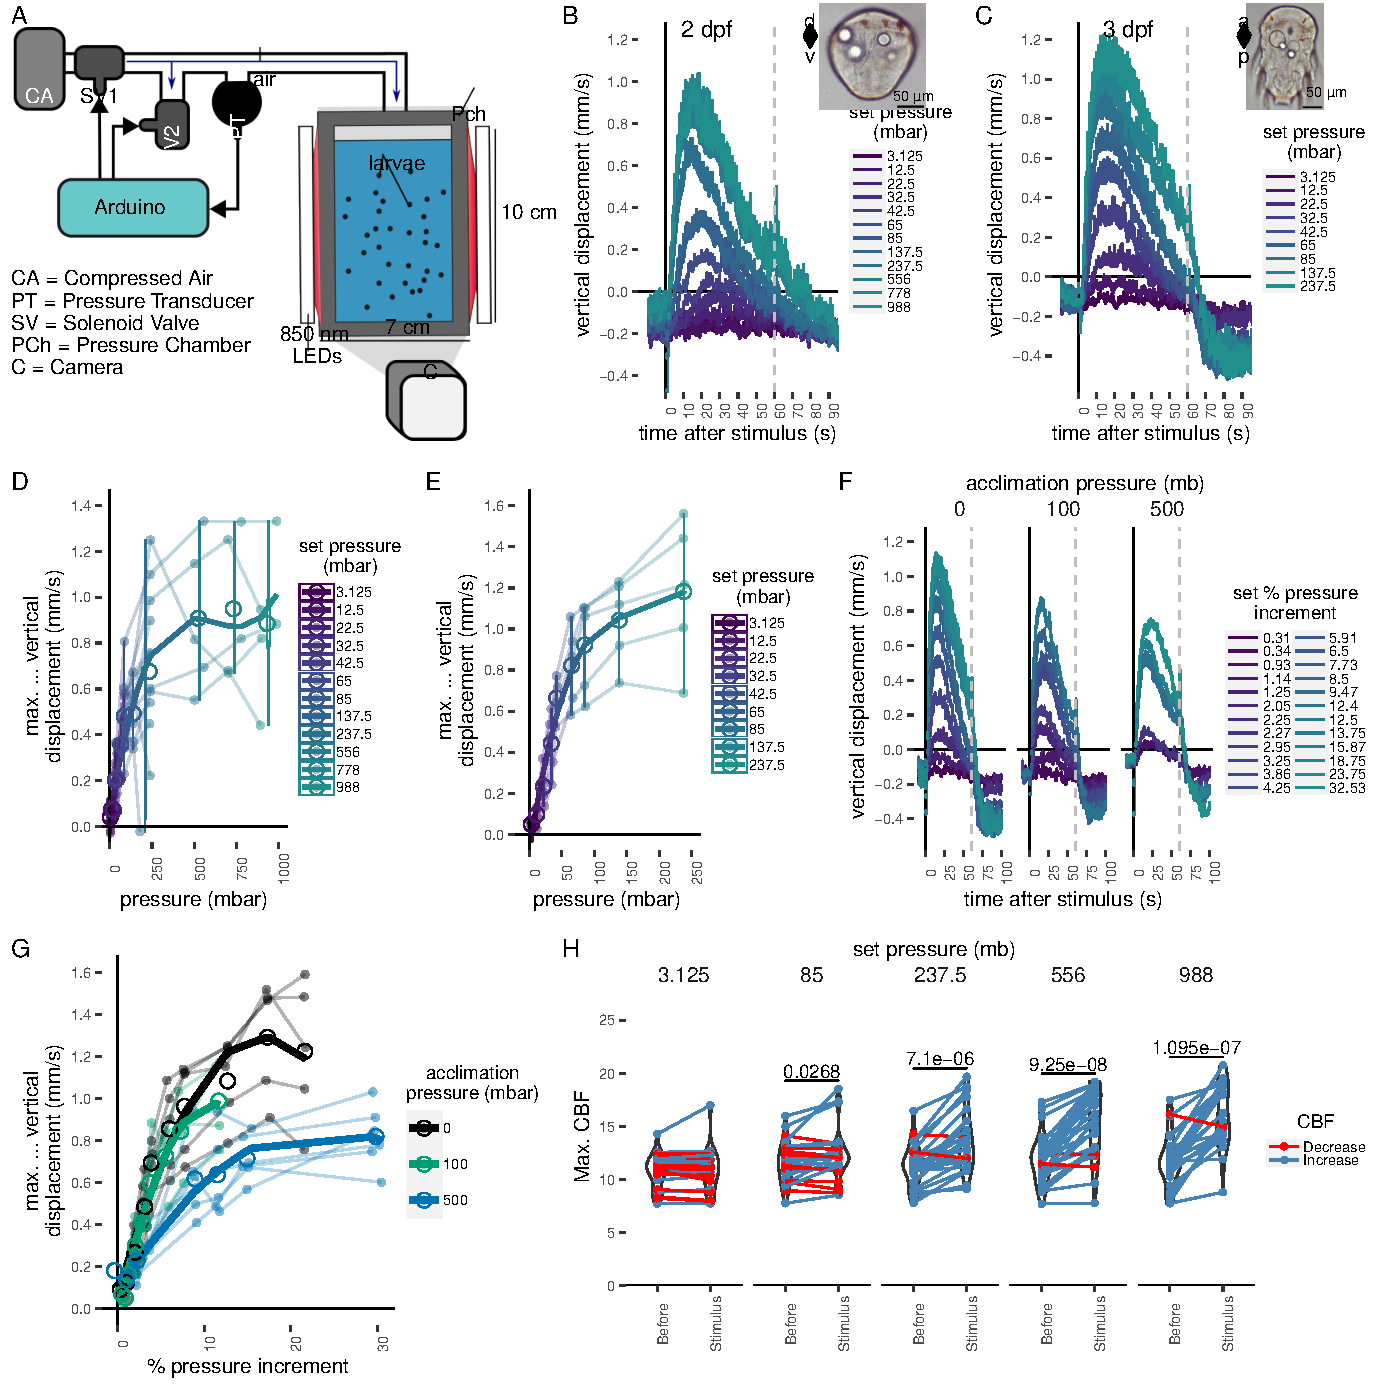
\includegraphics[width=38.89in]{Figures/Figure1} \caption{**Figure 1.** Pressure response in _Platynereis_ larvae. (A) Schematic of the behavioural setup used to stimulate larvae with controlled pressure levels. (B-C) Vertical displacement of (B) two-day-old and (C) three-day-old larvae (insets) as a function of time relative to different step increases in pressure. Dashed line at 60 s indicates the end of stimulation. Each data point is the average of 2 to 12 (B), or 4 to 5 (C) batches of larvae. (D-E) Maximum increase in relative vertical displacement of (D) two-day-old and (E) three-day-old larvae for each pressure level tested. Small filled circles represent individual data points, data points from the same batch are joined by lines. Larger open circles indicate the mean across all batches. (F) Vertical displacement of three-day-old larvae acclimated for ca. 10 min to either ambient pressure (0 mb, left), 100 mb (centre), or 500 mb (right) prior to the experiment. Lines are coloured by set fractional increments in pressure. (G) Maximum increase in relative vertical displacement of three-day-old larvae acclimated to 0 mb, 100 mb or 500 mb. The data are fitted with a saturation curve. 5 (0, 100 mb) or 6 (500 mb) batches tested in F—G. (H) Maximum ciliary beat frequency (CBF) that single larvae reached in the 30 s prior (category _Before_), or during the first 30 s (_Stimulus_) of the indicated increase in pressure. N = 18-22 larvae. Data points for the same larva are joined by lines. One-tailed paired t-test with Bonferroni correction testing for an increase in CBF; p-values < 0.05 are shown. Data in D, E and G were fitted with a 3<sup>rd</sup> (D, E) or a 2<sup>nd</sup> (G) order polynomial function. Figure 1---source data 1 (A,D), Figure 1---source data 2 (C,E), Figure 1---source data 3 (F-G),Figure 1---source data 4 (H).}\label{fig:unnamed-chunk-2}
\end{figure}

We used the maximal vertical displacement value (normalised to the mean
displacement per trial prior to stimulus presentation) to compare the
magnitude of responses as a function of pressure change. In both two-
and three-day-old larvae the responses were graded: higher pressure
levels led to higher maximal vertical displacement (Figure 1D--E).
Three-day-old larvae had a slightly lower sensitivity threshold (10-20
mbar) than two-day-old larvae (20-30 mbar) and their response plateaued
at lower pressure levels than that of two-day-old larvae (Figure 1B-E).
One-day-old larvae did not show a detectable response to even the
largest pressure levels tested (Figure 1---figure supplement 2A--B). The
straightness of trajectories also increased with increasing pressure
changes. This was due to narrower helical swimming paths under pressure,
visible in close-up videos (Figure 1---Supplement Video 2 \& Figure
1---Supplement Video 3). Three-day-old larvae also showed a diving
response upon the release of pressure (Figure 1B--C, F; Figure
1---figure supplement 1C--D). Two-day-old larvae stopped moving upwards
when the stimulus ended, but did not show an active diving response to
pressure OFF. To exclude the possibility that either the changes in the
partial pressure of gases due to the use of compressed air, or the
mechanical wave associated to the inflow of air was causing the upward
swimming behaviour, we also used a static column of water of different
heights to change pressure levels (Figure 1---figure supplement 2C). We
observed the same dependence of vertical displacement on the magnitude
of pressure change in this setup (Figure 1---figure supplement 2D-E).
Overall, our experiments uncovered a graded, saturable and highly
sensitive upward swimming ON response to increased pressure in
\emph{Platynereis} larvae and a diving OFF response (in three-day-old
larvae only).

\hypertarget{platynereis-larvae-respond-to-relative-changes-of-pressure}{%
\subsubsection{\texorpdfstring{\emph{Platynereis} larvae respond to
relative changes of
pressure}{Platynereis larvae respond to relative changes of pressure}}\label{platynereis-larvae-respond-to-relative-changes-of-pressure}}

Larvae may either detect absolute pressure levels, relative changes, or
the rate at which pressure changes
(\protect\hyperlink{ref-morgan_1984}{Morgan 1984}). To differentiate
between these possibilities, we first exposed larvae to linear increases
of pressure with rates between 0.05 mbar s-1 and 2.6 mbar s-1 (Figure
1---figure supplement 3A). We used a 2nd-degree polynomial function for
rate categories 0.3-0.7 mbar s-1 (ANOVA, p = 6.5e-3) and 0.9-1.3 mbar
s-1 (ANOVA, p= 5.8e-8 ), as it described the relationship between
vertical displacement and pressure more accurately than a simple linear
model. The difference between a linear and a 2nd-degree polynomial fit
was not significant for rates \textgreater{} 1.3 mbar s-1 (ANOVA,
p\textasciitilde{} 0.1). These results suggest that larvae compensate
for the increase in pressure by a corresponding increase in upward
swimming when rates of pressure increase are sufficiently high.

The linear response to a gradual increase in pressure suggests that
larvae detect changes in pressure, rather than absolute pressure levels.
To directly address this, we acclimated three-day-old larvae for ca. 10
min to either 100 mbar or 500 mbar pressure above the atmospheric level.
We then tested a range of randomized step-increases in pressure levels
(Figure 1---figure supplement 3D). After the acclimation period, the
distribution of larvae exposed to 100 mbar or 500 mbar was not different
from the larvae kept at ambient levels (two-sided Kolmogorov Smirnoff
test, 0--100 mbar: p = 0.915, 0--500 mbar: p = 0.0863) (Figure
1---figure supplement 3E--F). Upon step increase, larvae reacted with
graded upward swimming even if they were pre-exposed to 100 or 500 mbar
(Figure 1F). The sensitivity decreased when larvae were acclimated to
500 mbar (Figure 1G). When pressure was released at the end of the
increase trials, larvae pre-exposed to 500 mbar showed a downward
displacement followed by an upward displacement as soon as pressure was
increased back to the corresponding basal level (Figure 1---figure
supplement 3G). The downward displacement resembled the magnitude of the
diving response we observed for 3-day-old larvae (Figure 1---figure
supplement 3H).

Our experiments suggest that \emph{Platynereis} larvae react to relative
increases in pressure in a graded manner proportional to the magnitude
of the increase. The response is adaptable and occurs at very different
basal pressures (0 mbar or 500 mbar---corresponding to 5 m of water
depth). This hints at a pressure-gauge mechanism to regulate swimming
depth by compensating for vertical movements due to sinking (when cilia
are arrested (\protect\hyperlink{ref-veraszto2017a}{Verasztó et al.
2017})), downward swimming (e.g., during UV-avoidance
(\protect\hyperlink{ref-veraszto2018}{Verasztó et al. 2018})) or
down-welling currents (\protect\hyperlink{ref-genin2005a}{Genin et al.
2005}).

\hypertarget{ciliary-beat-frequency-increases-with-pressure}{%
\subsection{Ciliary beat frequency increases with
pressure}\label{ciliary-beat-frequency-increases-with-pressure}}

To understand the mechanism by which larvae regulate swimming in
response to an increase in pressure, we analysed the effect of pressure
on ciliary beating in the prototroch---the main ciliary band that
two-day-old and three-day-old \emph{Platynereis} larvae use to swim.
Individual two-day-old larvae were tethered to a glass cuvette from the
posterior end with a non-toxic glue previously used in
\emph{Platynereis} larvae
(\protect\hyperlink{ref-bezares-calderon2018}{Luis A. Bezares-Calderón
et al. 2018}). The cuvette was inserted into a custom-made pressure
vessel placed under a microscope. We recorded ciliary beating in
effective darkness (Figure 1---figure supplement 4A). Step increases in
pressure were applied for 60 sec in a randomized manner to levels
comparable to those used in batch experiments (Figure 1---figure
supplement 4B).

The mean ciliary beat frequency increased as soon as the step change in
pressure was applied, with larger step changes showing more noticeable
increases in beat frequency (Figure 1---figure supplement 4C, Figure
1---Supplement Video 4). The maximum ciliary beat frequency (max. CBF)
during the stimulus period showed a statistically significant increase
for all but the lowest pressure steps tested relative to the period
before the onset of the stimulus (85 mb p = 0.046, 237.5 mb p = 2.08
E-05, 556 mb p = 8.35 E-07, 988 mb p = 7.8 E-07; one-tailed paired
t-test with Bonferroni correction testing for an increase in CBF; Figure
1H). The related relative measure of maximum percent change (max.
∆\%CBF) also showed an increase under pressure (Figure 1---figure
supplement 4D). Overall, these data suggest that rapid upward swimming
under pressure is due to an increase in the beating frequency of
prototroch cilia that is proportional to the change in pressure.

\hypertarget{brain-ciliary-photoreceptor-cells-show-graded-activation-under-increased-pressure}{%
\subsection{Brain ciliary photoreceptor cells show graded activation
under increased
pressure}\label{brain-ciliary-photoreceptor-cells-show-graded-activation-under-increased-pressure}}

To identify the pressure-sensitive cells in \emph{Platynereis} larvae,
we developed an approach to couple imaging of neuronal activity~with
pressure increases (Figure 2A). We injected fertilised eggs with mRNA
encoding the calcium indicator GCaMP6s
(\protect\hyperlink{ref-chen2013}{Chen et al. 2013})---an indirect
reporter of neuronal activity---and embedded injected larvae in
low-melting agarose. Mounted larvae were introduced into a custom-built
microscopy chamber, where pressure could be increased using compressed
air. To provide morphological landmarks and to correct for Z-shifts
during imaging, we co-injected larvae with an mRNA encoding the
membrane-tagged reporter palmitoylated tdTomato.

\begin{figure}
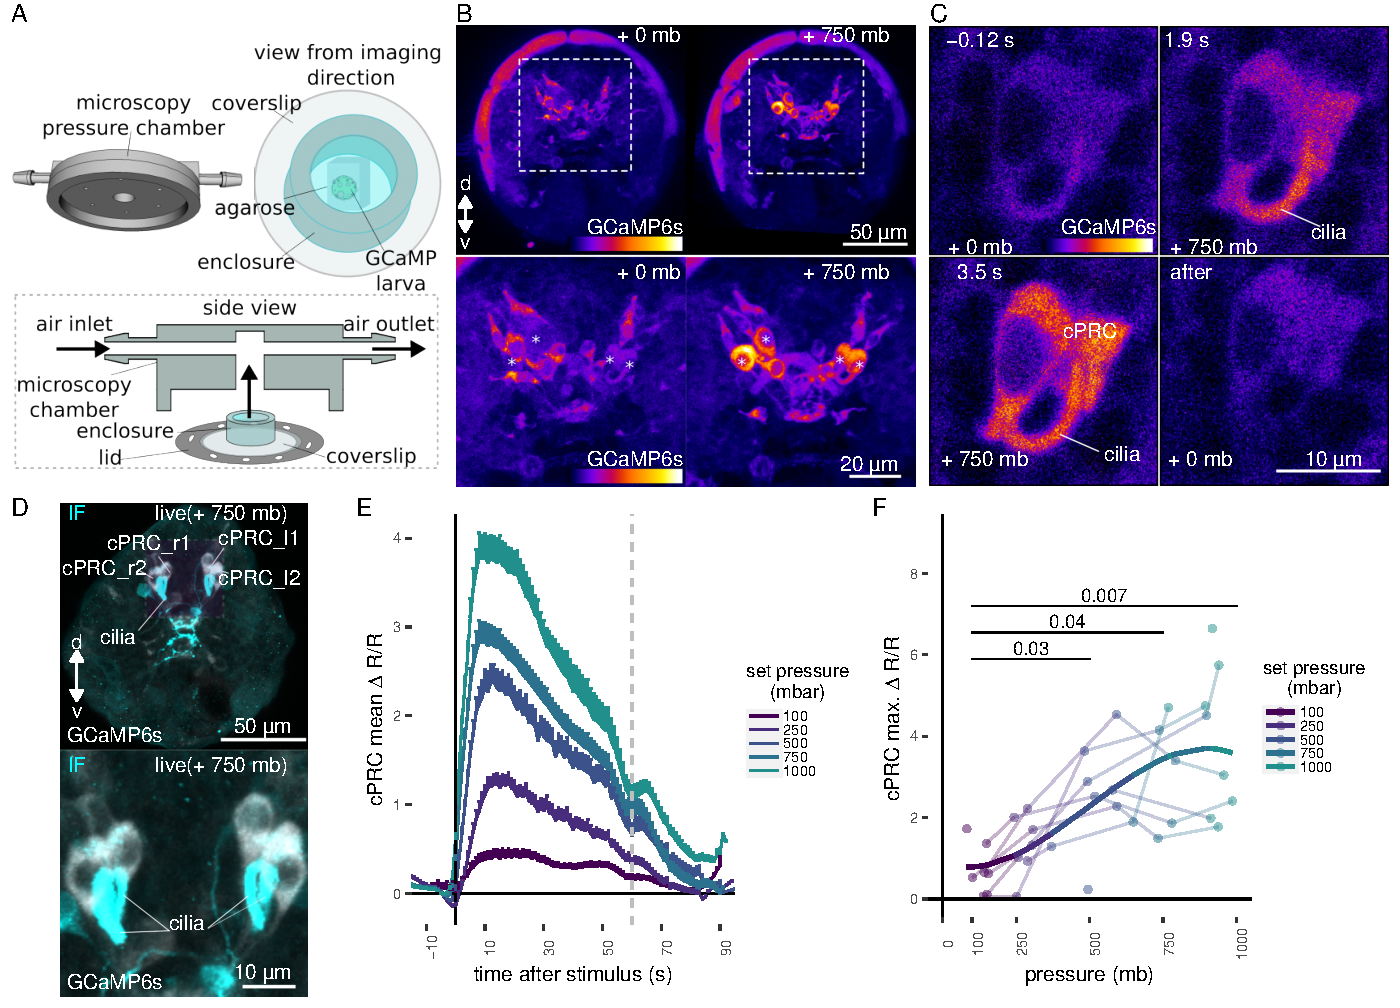
\includegraphics[width=38.89in]{Figures/Figure2} \caption{**Figure  2.** Ca²⁺ imaging of *Platynereis* larvae during pressure increases. (A) Ca²⁺ imaging preparation to analyse neuronal activation upon pressure stimulation. Left: side view of the 3D model of the microscopy pressure chamber. Right: Larvae embedded in agarose are placed on a round coverslip. An enclosure around the embedded larva serves to keep it under water. Bottom: the enclosed larva on the coverslip is inserted in the central hole of the chamber. A screwable lid secures the coverslip to the chamber and prevents air leaks. Pressure is increased with compressed air entering from one of the inlets. (B, top) Maximum intensity projection of a two-day-old larva injected with _GCaMP6s_ mRNA acquired before (left) or during (right) the pressure stimulus. (B, bottom) Enlarged views of the corresponding regions highlighted with dashed squares in the top panels. Asterisks mark the position of cell nuclei of the four cells activated by pressure. (C) Still images of a cPRC acquired at different time points relative to increase in pressure (t = 0, Figure 2---Supplement Video 1). The time points are indicated on the upper left of each panel. Pressure level is also indicated. (D) Max. intensity projection of a GCaMP6s Z-stack during raised pressure (white channel) and of a Z-stack of the same larva after immunofluorescence (IF) with NIT-GC2, a marker for cPRC cilia, and for serotonin (cyan channel). Anterior view in B–D. (E) Mean ∆R/R in cPRC_l1 across different step increases in pressure as a function of time of stimulation. Dashed line at 60 s marks the end of stimulus. N = 8 larvae. (F) Max. ∆R/R in cPRC_l1 as a function of pressure level. Data points from the same larva are joined by lines. Regression line fitting the data is also shown. One-tailed unpaired t-test with Bonferroni correction testing for an increase in Max. ∆R/R with pressure. p-values < 0.05 are shown. Figure 2---source data 1 (E-F). }\label{fig:unnamed-chunk-3}
\end{figure}

By imaging the entire larva before and during the pressure stimulus, we
found a group of four cells on the dorsal side of the brain that showed
consistent increases in GCaMP6s fluorescence when pressure increased
(Figure 2B; Figure 2---figure supplement 1). Time-lapse recordings of
these cells revealed that they had prominent cilia, which become visible
by the increase in GCaMP6s signal during pressure increase (Figure 2C,
Figure 2---Supplement Video 1). The position, number, size and
morphology of these cells closely matched to that of the previously
described brain ciliary photoreceptor cells (cPRCs)
(\protect\hyperlink{ref-arendt2004}{Arendt et al. 2004};
\protect\hyperlink{ref-Tsukamoto2017}{Tsukamoto et al. 2017};
\protect\hyperlink{ref-veraszto2018}{Verasztó et al. 2018}).
Immunostaining of the same larvae that were used for
Ca\textsuperscript{2+} imaging with an antibody raised against NIT-GC2,
a marker of cPRC cilia (\protect\hyperlink{ref-jokura2023}{Jokura et al.
2023}), followed by image registration directly confirmed that the four
cells activated under pressure were the cPRCs (Figure 2D).

To characterise the response of cPRCs to pressure, we applied a
randomised set of pressure increases (Figure 2---figure supplement 2A)
to two-day-old larvae injected with \emph{GCaMP6s} mRNA while recording
fluorescence changes in the four cPRCs. All four cPRCs responded to the
pressure levels tested (Figure 2E; Figure 2---figure supplement 2B--C).
This response---like that observed at the behavioural level---was graded
and increased proportionally to the pressure change (Figure 2E--2F;
Figure 2---figure supplement 2B--C, 2E). The difference in the response
between pressure levels was statistically significant for some of the
cPRCs (Figure 2F; Figure 2---figure supplement 2C). The calcium signal
also decreased rapidly after stimulus onset. Therefore, cPRCs may be
able to directly encode the intensity of the stimulation in their
activity, reflected in their internal Ca\textsuperscript{2+} levels, and
adapt to pressure levels. The unique sensory morphology and
pressure-induced Ca\textsuperscript{2+} dynamics make the cPRCs
candidate pressure receptors.

An additional unpaired sensory cell on the dorsal side was also
activated in some of the trials (Figure 2---figure supplement 1, green
asterisk). We refer to this cell here as SN\textsuperscript{d1\_unp} (by
position and morphology it corresponds to the neurosecretory cell
SN\textsuperscript{YFa+} (\protect\hyperlink{ref-williams2017}{Williams
et al. 2017})). At 750 mb, this cell responded by a transient but robust
increase at stimulation onset, but ∆R/R dropped to basal values before
the end of the stimulus, unlike the cPRC response (Figure 2---figure
supplement 2D). SN\textsuperscript{d1\_unp} (SN\textsuperscript{YFa+})
may also contribute to the pressure response, although it is less
sensitive than cPRCs and has very few synapses
(\protect\hyperlink{ref-williams2017}{Williams et al. 2017}).

Another indirect observation that is consistent with cPRCs being the
primary pressure receptors is that one-day-old larvae that lack
differentiated cPRCs (\protect\hyperlink{ref-fischer2010}{Fischer,
Henrich, and Arendt 2010}) do not respond to pressure (Figure 1---figure
supplement 2A).

\hypertarget{c-opsin-1-mutants-have-a-reduced-pressure-response}{%
\subsection{\texorpdfstring{\emph{c-opsin-1} mutants have a reduced
pressure
response}{c-opsin-1 mutants have a reduced pressure response}}\label{c-opsin-1-mutants-have-a-reduced-pressure-response}}

cPRCs express ciliary-opsin-1 (c-ops-1), which forms a UV-absorbing
photopigment (\protect\hyperlink{ref-arendt2004}{Arendt et al. 2004};
\protect\hyperlink{ref-Tsukamoto2017}{Tsukamoto et al. 2017};
\protect\hyperlink{ref-veraszto2018}{Verasztó et al. 2018}). Knocking
out the \emph{c-ops-1} gene abolishes a UV-avoidance response in
\emph{Platynereis} larvae (\protect\hyperlink{ref-veraszto2018}{Verasztó
et al. 2018}). As cPRCs respond to pressure increases, we tested whether
\emph{c-ops-1} knockout mutants (\emph{c-ops-1\textsuperscript{∆8/∆8}})
also showed a defect in the pressure response.

A range of step increases in pressure were applied to single batches of
either wild-type (WT) or \emph{c-ops-1\textsuperscript{∆8/∆8}}
three-day-old larvae (Figure 3---figure supplement 1A). The assays were
carried out in a smaller pressure vessel (height: \textasciitilde4 cm),
to allow consistent imaging of the fewer mutant larvae available. The
swimming speed of \emph{c-ops-1\textsuperscript{∆8/∆8}} mutant larvae
was not significantly different from \emph{WT} larvae (p = 0.118,
unpaired Wilcoxon test for lower speed in mutants; Figure 3---figure
supplement 1B). \emph{c-ops-1\textsuperscript{∆8/∆8}} larvae responded
in a graded manner to increases in pressure by upward swimming (Figure
3A; Figure 3---figure supplement 1C). However, their response was weaker
than the response of age-matched \emph{WT} larvae (Figure 3---figure
supplement 1C). An ANOVA comparison showed that a model considering the
genotype better explained the data than a model without this variable,
for either a simple or a polynomial linear regression model (p-values =
9.98e⁻⁰⁷ and 9.92e⁻⁰⁶, respectively). Ciliary beating prior to pressure
increase was not significantly different between
\emph{c-ops-1\textsuperscript{∆8/∆8}} and WT larvae (p = 0.835, unpaired
Wilcoxon test for lower CBF in mutants; Figure 3---figure supplement
1D). Upon pressure increases, CBF in
\emph{c-ops-1\textsuperscript{∆8/∆8}} larvae showed a significant
increase to the three highest pressure levels tested (237.5 mb p =
0.014, 556 mb p = 9.7 E-05, 988 mb p = 6.35 E-05; one-tailed paired
t-test with Bonferroni correction testing for an increase in CBF; Figure
3B). \emph{c-ops-1\textsuperscript{∆8/∆8}} larvae also showed
significant increases in max. ∆\%CBF as the pressure stimulus was
increased (Figure 3---figure supplement 1E; compare to the WT data in
Figure 3B), with no significant difference in the increase to WT larvae
(Figure 3---figure supplement 1F). In summary,
\emph{c-ops-1\textsuperscript{∆8/∆8}} larvae can still respond to
changes in pressure in a graded manner, but the response is weaker than
in \emph{WT} larvae, both at the population and at the single-larva
levels. This indicates that c-opsin-1 is not directly required for the
pressure response, but its absence leads to a weakened response to
pressure.

\begin{figure}
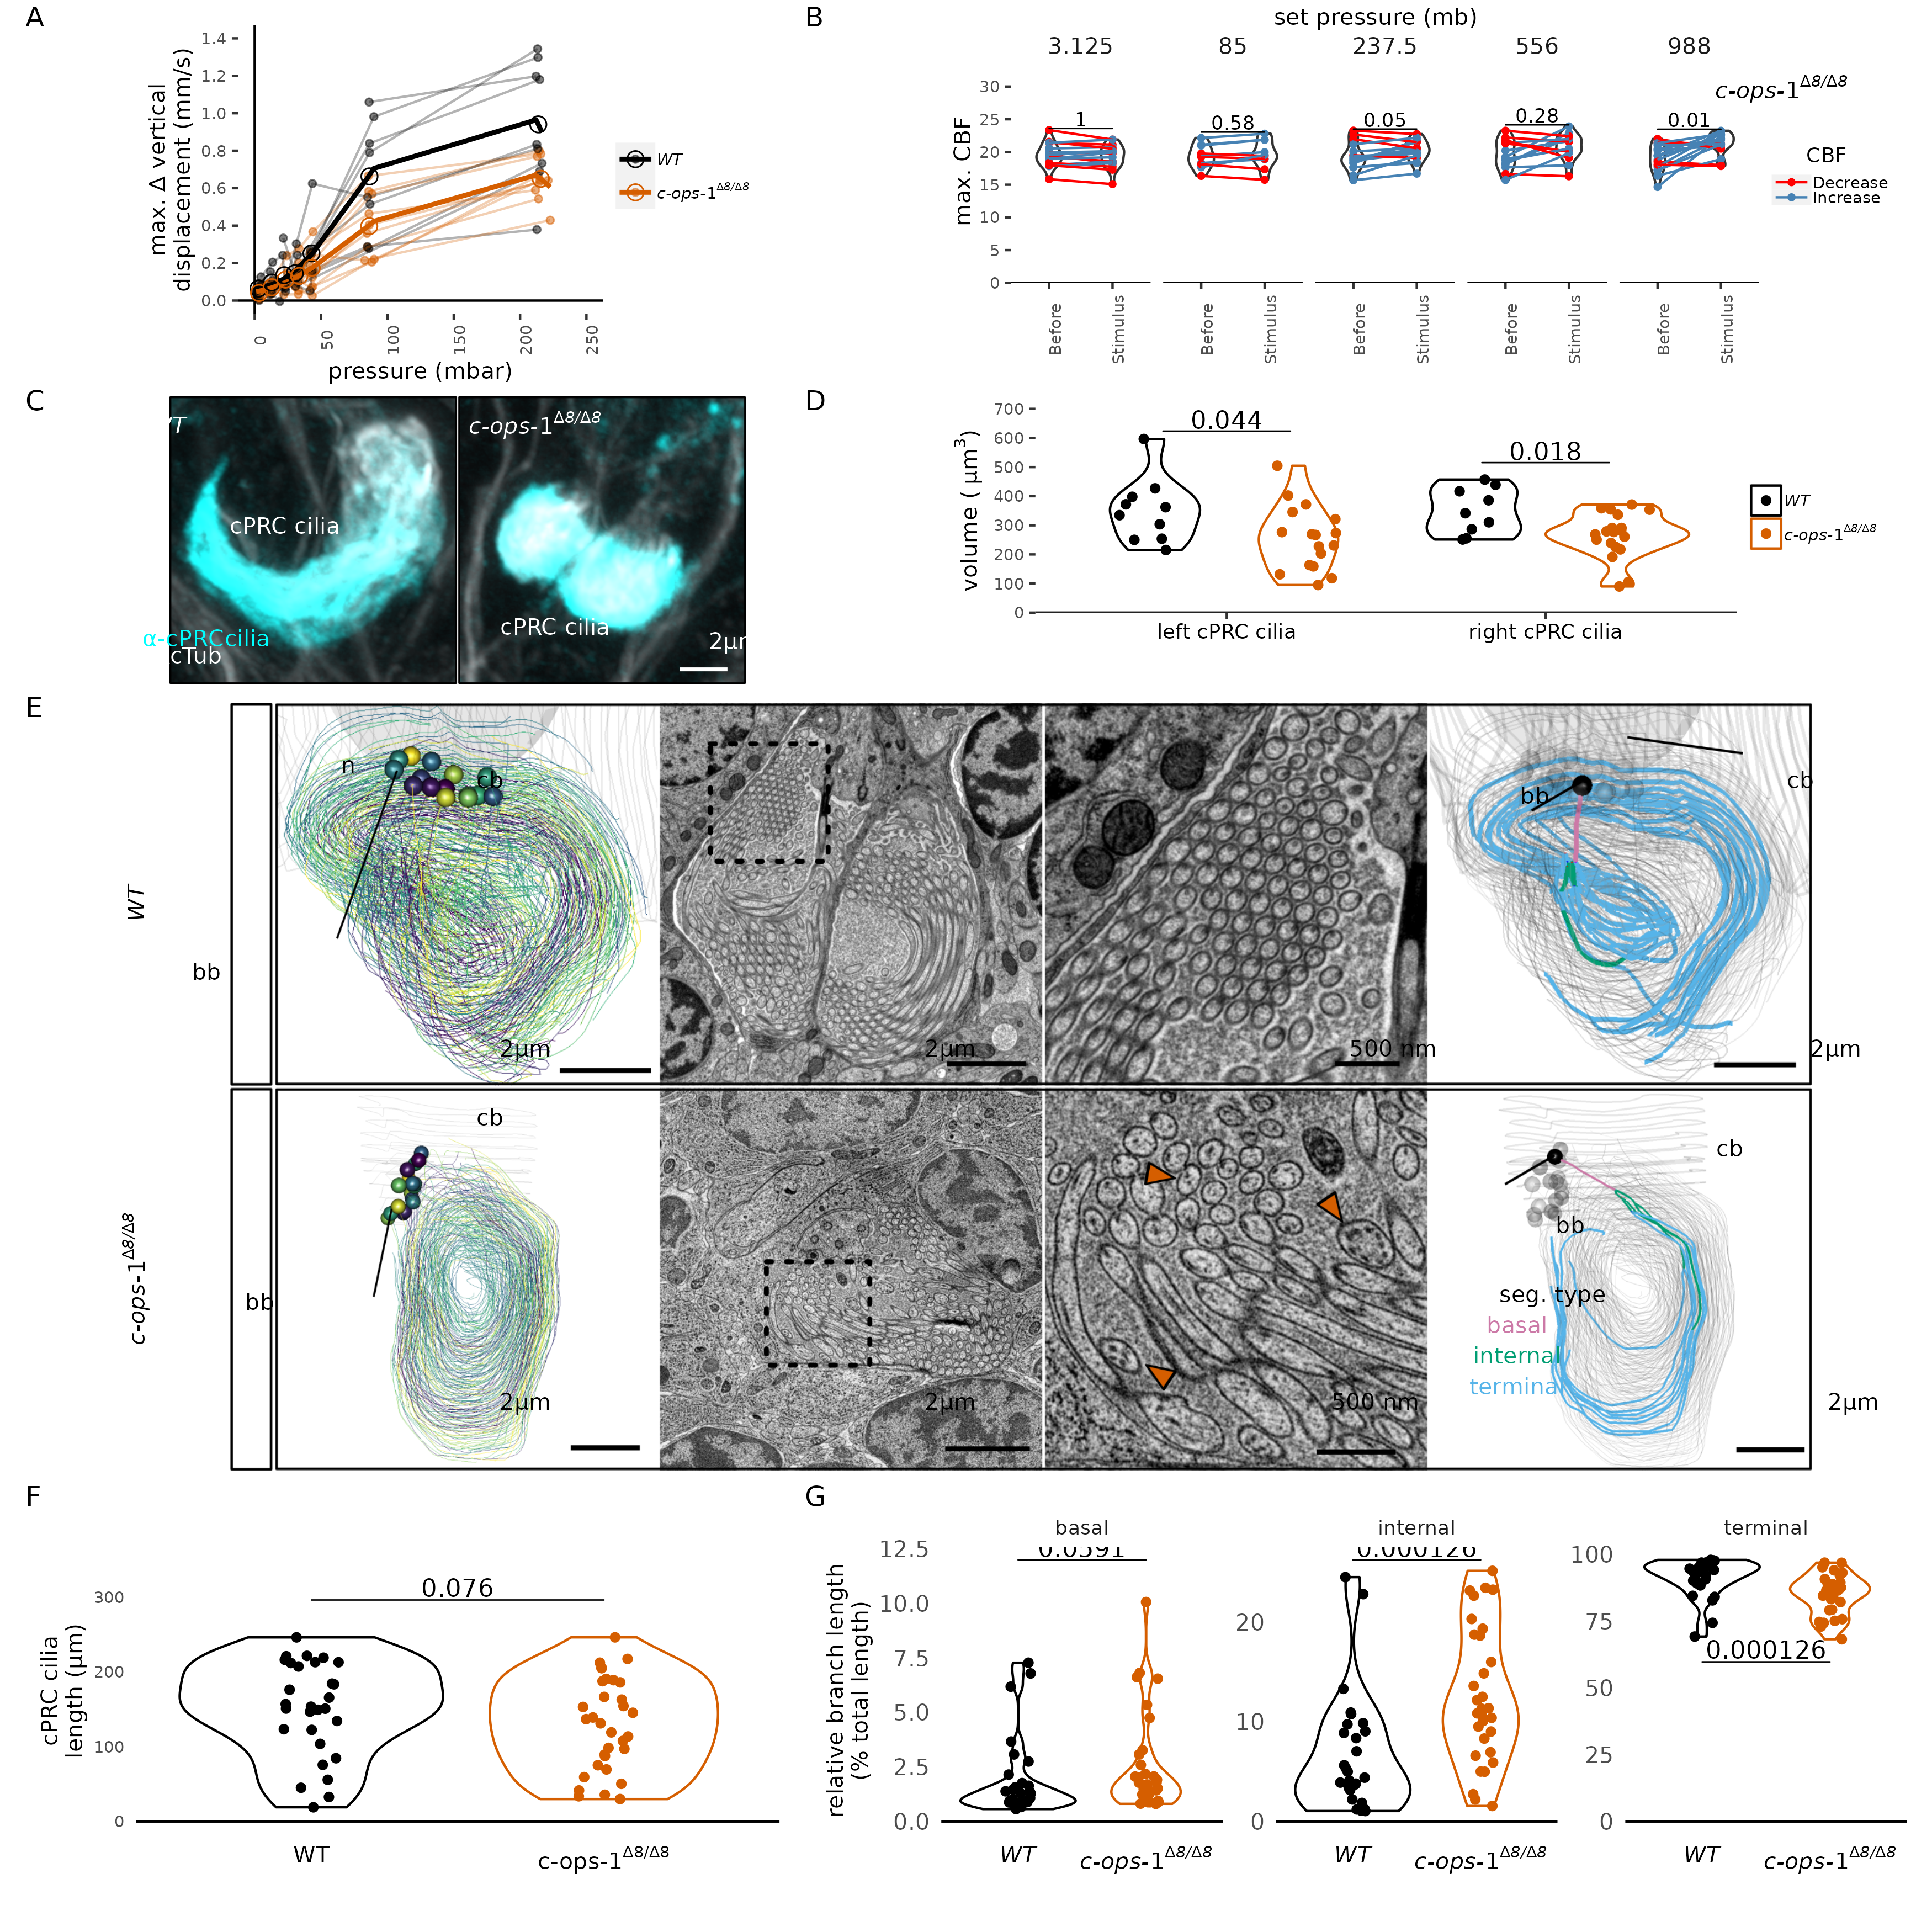
\includegraphics[width=48.61in]{Figures/Figure3} \caption{**Figure 3.** _c-ops-1^∆8/∆8^_ larvae show a weaker response to pressure and have structural defects in cPRC cilia. (A) Maximum change in vertical displacement of  _WT_ and  _c-ops-1^∆8/∆8^_ three-day-old larvae for each pressure step-change tested. Data points from the same batch are joined by lines. Larger open circles indicate the mean value. Thicker solid lines show the regression model predictions. N= 7-9 ( _c-ops-1^∆8/∆8^_), N = 8-10 ( _WT_) batches. (B) Max. CBF that individual  _c-ops-1^∆8/∆8^_ larvae reached in the 30 s prior (_Before_), or during the first 30 s of the indicated increase in pressure (_Stimulus_). Data points for the same larva are joined by lines. One-tailed paired t-test with Bonferroni correction testing for an increase in CBF; all p-values are shown. N = 10—17 larvae. (C-D) cPRC ciliary volume measured for each pair of cPRC cilia on the left and right body sides in two-day-old  _WT_ and _c-ops-1^∆8/∆8^_ larvae. Volumes were measured using the signal of the cPRC cilia antibody (α-cPRCcilia). (C)  Maximum intensity projections of IF stainings used for quantifying cPRC cilary volume. (D) cPRC ciliary volume distribution sorted by genotype and body side. One-tailed unpaired t-test with Bonferroni correction testing for a decrease in ciliary volume in mutant larvae. p-values < 0.05 are shown. N = 9—10 ( _WT_), 17—19 (_c-ops-1^∆8/∆8^_) larvae. (E) Morphology of cPRC cilia in 3 day-old _WT_ (top row) and _c-ops-1^∆8/∆8^_ (bottom row) larvae reconstructed by serial EM. Reconstructions of cPRC cilia are shown in the left-most panels. A representative micrograph of the EM data used for the reconstructions is shown in the adjacent panels. Dashed squares in these images mark the regions shown in the enlarged views to the right. Orange arrowheads point to cilia with more than one microtubule dublets. In the right-most panels, the branches of single cPRC cilia are coloured by Strahler order (Str. order). Branches with higher Str. orders originate closer to the basal body (bb). The remaining cPRC cilia are coloured in grey. cb: cell body; n: nucleus; bb: basal body. Figure 3---source data 1 (A), Figure 1---source data 4 (B), Figure 3---source data 2 (D).}\label{fig:unnamed-chunk-4}
\end{figure}

\hypertarget{c-opsin-1-mutants-have-defects-in-cprc-cilia}{%
\subsection{\texorpdfstring{\emph{c-opsin-1} mutants have defects in
cPRC
cilia}{c-opsin-1 mutants have defects in cPRC cilia}}\label{c-opsin-1-mutants-have-defects-in-cprc-cilia}}

The reduced response of \emph{c-ops-1\textsuperscript{∆8/∆8}} larvae to
pressure may stem from morphological defects of the cPRC sensory cilia
in these mutants. We used stainings with acetylated tubulin and NIT-GC2,
an antibody specifically marking cPRC cilia (see Figure 2D) to measure
the volume of the ciliary compartment in \emph{WT} and
\emph{c-ops-1\textsuperscript{∆8/∆8}} larvae (Figure 3C; Figure
3---figure supplement 1G). Volumetric imaging in two-day-old larvae
stained with these antibodies revealed that the cPRC ciliary compartment
in \emph{c-ops-1\textsuperscript{∆8/∆8}} larvae was significantly
smaller than in age-matched \emph{WT} larvae (p = 0.044 and 0.018 for
left and right ciliary compartments, one-tailed unpaired t-test with
Bonferroni correction; Figure 3D). In some cases, cPRC ciliary
compartments were drastically reduced, albeit never completely absent in
all four cells (Figure 3---figure supplement 1F). A reduced ciliary
compartment may underlie the weaker responses of
\emph{c-ops-1\textsuperscript{∆8/∆8}} larvae to pressure.

To further investigate the morphological defects of cPRC sensory cilia
in \emph{c-ops-1\textsuperscript{∆8/∆8}} larvae, we reconstructed the
cPRC ciliary structure of a mutant larva using volume electron
microscopy. We compared this reconstruction to a volume EM datataset of
cPRC cilia from a three-day-old \emph{WT} larva previously reported
(\protect\hyperlink{ref-veraszto2018}{Verasztó et al. 2018}). The two
\emph{WT} cPRCs reconstructed have 14 to 15 ramified cilia tightly
wrapped on themselves (Figure 3E, top row, Figure 3---Supplement Video
1). Branching occurs close to the basal body, soon after cilia protrude
from the cell body. Most branches inherit an individual microtubule
doublet. The 15 to 17 cilia of the two cPRCs reconstructed in a
\emph{c-ops-1\textsuperscript{∆8/∆8}} larva revealed a more sparsely
packed structure (Figure 3E, bottom row; Figure 3---figure supplement
1A, Figure 3---Supplement Video 2). Mutant cilia are not significantly
shorter than WT cPRC cilia (p = 0.076, Wilcoxon test for longer WT
cilia, Figure 3F). However, we noticed when comparing cross-sections of
each genotype that individual branches of mutant cPRC cilia often
contained more than one microtubule doublet (arrowheads in Figure 3E;
Figure 3---figure supplement 2A). This suggests that cPRC cilia of
\emph{c-ops-1\textsuperscript{∆8/∆8}} larvae have alterations in
branching morphology. We indeed found that the terminal branches of
cilia in the mutant are significantly shorter (p = 1.26 E-04 Wilcoxon
test for shorter branches in the mutant, Figure 3G, right-most plot),
while internal branches are longer than those in the \emph{WT} (p = 1.26
E-04; Wilcoxon test for longer branches in the mutant, Figure 3G, middle
plot). Basal branches also tended to be larger, but no statistically
significance can be concluded (p = 0.06, Wilcoxon test for longer
branches in the mutant, Figure 3G, left-most plot). This result supports
the former observation that branching occurs more distally to the basal
body in \emph{c-ops-1\textsuperscript{∆8/∆8}} larvae. Longer internal
branches in mutant cPRC cilia would also explain the presence of ciliary
profiles with more than one microtubule doublet (Figure 3---figure
supplement 2A).

Overall, our physiological and genetic analyses suggest that the brain
cPRCs act as graded and fast-adapting pressure receptors. In
\emph{c-ops-1\textsuperscript{∆8/∆8}} larvae, the ciliary compartment is
smaller and shows morphological defects, revealing a genetic requirement
for c-opsin-1 in the establishment of the sensory compartment and
supporting the idea that the cPRC ciliary compartment is the site of
pressure transduction.

\hypertarget{synaptic-transmission-from-serotonergic-ciliomotor-neurons-mediates-pressure-induced-increases-in-ciliary-beating}{%
\subsection{Synaptic transmission from serotonergic ciliomotor neurons
mediates pressure-induced increases in ciliary
beating}\label{synaptic-transmission-from-serotonergic-ciliomotor-neurons-mediates-pressure-induced-increases-in-ciliary-beating}}

The complete synaptic wiring diagram of the cPRCs was previously
reported from an electron microscopy volume of a three-day-old larva
(Figure 4A-B; Verasztó et al.
(\protect\hyperlink{ref-veraszto2018}{2018})). The shortest neuronal
path from cPRCs to the prototroch involves a feed-forward loop from the
cPRCs to two types of postsynaptic interneurons, the INNOS and the
INRGWa cells (Figure 4B). INRGWa cells in turn synapse on a pair of head
serotonergic ciliomotor neurons (Ser-h1). Ser-h1 cells directly
innervate the prototroch ciliary band and synapse on the MC head
cholinergic ciliomotor neuron (Figure 4B). Ser-h1 cells are thought to
promote ciliary beating by directly releasing serotonin onto the ciliary
band cells and indirectly by inhibiting the cholinergic MC neuron that
is required to arrest ciliary beating
(\protect\hyperlink{ref-veraszto2017a}{Verasztó et al. 2017}).

To directly test the involvement of the Ser-h1 cells in the pressure
response, we used a genetic strategy to inhibit synaptic release from
serotonergic neurons. We used transient transgenesis to drive the
expression of the synaptic inhibitor tetanus-toxin light chain (TeTxLC)
(\protect\hyperlink{ref-sweeney1995}{Sweeney et al. 1995}) under the
promoter of \emph{tryptophan hydroxylase} (\emph{TPH}), a marker of
serotonergic neurons (\protect\hyperlink{ref-veraszto2017a}{Verasztó et
al. 2017}). The \emph{TPH} promoter labels the head Ser-h1 and other
serotonergic cells including the Ser-tr1 trunk ciliomotor neurons. Of
the cells labelled with this promoter, only Ser-h1 is postsynaptic to
cPRCs and provides strong innervation to the prototroch cells and the MC
cell (\protect\hyperlink{ref-veraszto2017a}{Verasztó et al. 2017}).

The construct (Figure 4C) drives the expression of both TeTxLC and an
HA-tagged palmitoylated tdTomato reporter, separated by P2A, a
self-cleaving peptide previously used in \emph{Platynereis}
(\protect\hyperlink{ref-bezares-calderon2018}{Luis A. Bezares-Calderón
et al. 2018}). The mosaic expression of this construct resulted in the
labeling of different subsets of serotonergic neurons. We selected
animals showing labelling in Ser-h1 (most larvae were also labelled in
Ser-tr1 and other unidentified serotonergic cells). We confirmed the
expression of the transgene in Ser-h1 by immunostaining against the
HA-tag of Palmi-tdTomato (Figure 4D). Larvae expressing TeTxLC in Ser-h1
showed an increase in CBF only at the highest pressure used (988 mb p =
0.004; one-tailed paired t-test with Bonferroni correction testing for
an increase in CBF; Figure 4E, bottom row). Larvae injected with a
control plasmid expressing only Palmi-tdTomato but not TeTxLC in Ser-h1
(Figure 4C) showed a significant increase in CBF at the three highest
pressure levels applied (237.5 mb p = 0.023, 556 mb p = 0.009, 988 mb p
= 0.004; one-tailed paired t-test with Bonferroni correction testing for
an increase in CBF; Figure 4E, top row; Figure 4---figure supplement
1A). The metric max. ∆\%CBF was not significantly different between
control and TeTxLC-injected larvae (Figure 4---figure supplement 1B).
These results indicate that TeTxLC-mediated inhibition of
Ser-h-1---albeit incomplete and in most cases limited to one of the two
cells---leads to a noticeable dampening of the pressure response at the
level of the ciliary band. This suggests that synaptic release from
serotonergic neurons is required to increase ciliary beating upon
pressure increase. Our data support the model that Ser-h1 neurons, and
no other serotonergic cells, are specifically required for this
response, because this cell type was labelled in all animals tested and
these cells directly innervate the prototroch.

\begin{figure}
\includegraphics[width=38.89in]{Figures/Figure4} \caption{**Figure 4.** TeTxLC expression in Ser-h1 neurons inhibits CBF increase during pressure. (A-B) Volume EM reconstruction (A) of the cells in the cPRC synaptic circuit (B). cPRCs synpase in the middle of the brain on both INNOS and INRGWa neurons. INRGWa cells synapse on Ser-h1 neurons, which directly innervate the ciliary band and also target the MC cell. Only the cells in the shortest path to the prototroch are included.  (C) Schematic of the gene constructs used to test the role of Ser-h1 in the pressure response. The TPHp::tdT construct drives expression of the reporter protein Palmi-tdTomato in Ser-h1 and other serotonergic neurons. It was used as a control. The TPHp::tdT-P2A-TeTxLC construct expresses Palmi-tdTomato and the synaptic blocker TeTxLC as a fusion that gets post-translationally self-cleaved by the P2A peptide. (D) Maximum intensity projections of a larva injected with the TPHp::tdT-P2A-TeTxLC construct and stained with α-HA. Ser-h1 was labelled in this animal. Anterior view. (E) Max. CBF that single larvae reached in the 30 s prior (_Before_), or during the first 30 s of the indicated increase in pressure (_Stimulus_). Data points for the same larva are joined by lines. Larvae were injected either with the control plasmid TPHp::tdT (top row, N = 14-16 larvae), or with the TPHp::tdT-P2A-TeTxLC plasmid (bottom row, N = 13-16 larvae). One-tailed paired t-test with Bonferroni correction testing for an increase in CBF; p-values < 0.05 are shown. Figure 4---source data 1 (E).}\label{fig:unnamed-chunk-5}
\end{figure}

\hypertarget{discussion}{%
\subsection{Discussion}\label{discussion}}

This work provides insights into the neuronal mechanisms of pressure
sensation and response in a marine planktonic larva. Our findings
suggest that increases in pressure, either due to the larva's own
actions (sinking or diving) or to downwelling currents, lead to the
activation of the sensory cPRCs (Figure 5). The activation is
proportional to the magnitude of pressure change and leads to the
activation of the downstream circuit that converges onto the Ser-h1
neurons and ultimately leads to increased ciliary beating. The Ser-h1
cells could secrete serotonin (5-HT) onto the ciliary band, which from
pharmacological assays is known to increase ciliary beat frequency
(\protect\hyperlink{ref-veraszto2017a}{Verasztó et al. 2017}). Ser-h1
neurons may simultaneously inhibit the cholinergic ciliomotoneuron MC
neuron (\protect\hyperlink{ref-veraszto2017a}{Verasztó et al. 2017}),
thereby preventing ciliary arrests while the larva tries to compensate
for the increased pressure.

\begin{figure}
\includegraphics[width=56.21in]{Figures/Figure5} \caption{**Figure 5.** The pressure response as a depth-retention mechanism mediated by the ciliary photoreceptor-cell circuit. (Top) *Platynereis* larvae maintain their position in the water column by controlling the beating dynamics of the ciliary band (t = 0, no net change in depth, ∆ depth = 0). A sufficiently rapid increase in depth (at t = 1) caused by intrinsic or extrinsic factors would lead to an increase in hydrostatic pressure. The change in depth relative to the previous state (∆ depth 1 or ∆ depth 2) will be perceived by the larva, which will try to counteract this change by increasing ciliary beat frequency of the prototroch, leading to upward swimming (at t = 2) until the pressure returns to the level previously experienced. A smaller change in pressure (∆ depth 1) will lead to a smaller increase in CBF (CBF 1, light green arrow) than a larger change (CBF 2). (Middle) Changes in pressure are sensed by the cPRCs. These sensory cells are activated in a graded manner according to the change in pressure. (Bottom) cPRCs signal via a postsynaptic circuit including the INRGWa and INNOS interneurons to the Ser-h1 neurons. Activation of these serotonergic neurons is required to increase ciliary beating directly on the prototroch cells and indirectly by inhibiting the MC neuron (CBF 1 or CBF2) proportional to the change in pressure.}\label{fig:unnamed-chunk-6}
\end{figure}

Our proposed depth-retention model complements a previouslz reported
spectral depth-gauge mechanism in the \emph{Platynereis} larva based on
its ability to respond to UV and green light
(\protect\hyperlink{ref-veraszto2018}{Verasztó et al. 2018}). As
previously hypothesized for other planktonic larvae
(\protect\hyperlink{ref-sulkin_1984}{Sulkin 1984}), pressure sensing in
\emph{Platynereis} may operate through negative feedback to retain a
particular depth, while light as a more variable stimulus could drive
intensity and wavelength-dependent changes in the vertical position of
larvae. Our unpublished results indeed suggest that green light
determines the direction of swimming and can override upward swimming
induced by pressure, which only influences the speed of swimming (LABC
and GJ, unpublished).

Our unexpected finding that ciliary photoreceptors, previously shown to
be sensitive to UV and green light
(\protect\hyperlink{ref-veraszto2018}{Verasztó et al. 2018}), are also
activated by pressure increase suggests that the integration of light
and pressure could begin at the sensory level in a single cell type. UV
light activates the cPRCs to induce downward swimming while pressure
increases induce upward swimming. The calcium dynamics of cPRCs depends
on the stimulus applied and may therefore underlie the mechanism by
which the cells decode and transmit a sensory signal to the downstream
circuit. UV induces a transient increase and subsequent drop in
Ca\textsuperscript{2+} levels followed by a sharp increase that persists
even after UV stimulation ends. In contrast, pressure induces a
transient increase in Ca\textsuperscript{2+} levels that terminates with
the stimulus. These observations suggest that the integration of light
and mechanical cues already occurs at the sensory-cell level. The
different activation dynamics may lead to the release of different
neurotransmitter and neuromodulator cocktails (cPRCs are cholinergic,
GABAergic, adrenergic and peptidergic
(\protect\hyperlink{ref-williams2017}{Williams et al. 2017};
\protect\hyperlink{ref-randel2014}{Randel et al. 2014};
\protect\hyperlink{ref-tessmar-raible2007}{Tessmar-Raible et al. 2007}))
and different activation patterns in the postsynaptic cells. Similar
integration can occur in \emph{Drosophila} larvae, where UV/blue light
and noxious mechanical stimuli are detected by the same sensory neuron
that together with other cells converges onto a circuit processing
multisensory stimuli (\protect\hyperlink{ref-imambocus2022}{Imambocus et
al. 2022}). In \emph{Platynereis}, other sensory cells (e.g., the
SN\textsuperscript{d1\_unp} cells; figure supplement 5) may contribute
to distinguishing the nature of the stimulus.

The cellular and molecular mechanisms by which cPRCs sense and transduce
changes in hydrostatic pressure deserve further enquiry. The mechanism
may involve the differential compression of microtubules along each
ciliary branch (\protect\hyperlink{ref-li2022a}{Li et al. 2022};
\protect\hyperlink{ref-nasrin2021}{Nasrin et al. 2021}), or differential
displacement of fluid inside the cilium
(\protect\hyperlink{ref-bell2008}{Bell 2008}). The cPRCs have a unique
multiciliated structure and are embedded in a protected environment
different from fluid-exposed cilia such as hydrodynamic mechanosensory
cilia (\protect\hyperlink{ref-bezares-calderon2018}{Luis A.
Bezares-Calderón et al. 2018}). These features are hard to reconcile
with current models of ciliary mechanosensation (e.g., see review by R.
Ferreira et al. (\protect\hyperlink{ref-ferreira2019}{2019})) . Instead,
the mechanism of pressure sensation at work in cPRCs may share more
similarities with non-neuronal cells detecting pressure, such as
chondrocytes (\protect\hyperlink{ref-pattappa2019}{Pattappa et al.
2019}) and trabecular meshwork cells
(\protect\hyperlink{ref-luo2014}{Luo et al. 2014}).

The molecular mechanisms of pressure detection remain unclear.
Components of the phototransduction cascade may be involved in pressure
sensation. Our results indicate that the ciliary opsin required for
detecting UV light is not essential for pressure sensation. This
molecule rather indirectly affects the ability of cPRCs to sense
pressure by contributing to the development or maintenance of a ramified
ciliary sensory structure. The structural role of opsins for shaping
ciliary cell morphology has also been reported in other photoreceptor
and mechanoreceptor cells (\protect\hyperlink{ref-lem1999}{Lem et al.
1999}; \protect\hyperlink{ref-zanini2018}{Zanini et al. 2018}). The
direct transducer of pressure may be a TRP channel. TRP channels can
signal downstream of opsins in phototransduction cascades and have been
postulated as the ultimate integrators of sensory stimuli
(\protect\hyperlink{ref-liu2015}{Liu and Montell 2015}).
Mechanosensitivity has also recently been reported for vertebrate rods
(\protect\hyperlink{ref-bocchero2020}{Bocchero et al. 2020}), including
the activation of these ciliary photoreceptors by pressure
(\protect\hyperlink{ref-pang2021}{Pang, Gao, and Wu 2021}). The cellular
and molecular mechanisms behind this sensitivity are still unclear, but
TRP or Piezo channels were suggested to be involved
(\protect\hyperlink{ref-bocchero2020}{Bocchero et al. 2020}).

The mechanism by which cPRCs detect pressure in \emph{Platynereis} may
also characterise the few other cases of pressure sensors based on
ciliated sensory cells (the crab statocyst, and the dog hair cells)
(\protect\hyperlink{ref-fraser_2002}{Peter J. Fraser and Shelmerdine
2002}; \protect\hyperlink{ref-fraser_1994}{Peter J. Fraser and Macdonald
1994}). Multiciliated pressure receptors may be widespread in
zooplankton, as cells with a morphology similar to the cPRCs have been
observed in species across the animal phylogeny
(\protect\hyperlink{ref-hernandez-nicaise1984}{Hernandez-Nicaise 1984}.;
\protect\hyperlink{ref-eakin1970}{Eakin and Kuda 1970};
\protect\hyperlink{ref-baatrup1982}{Baatrup 1982}), reviewed in
(\protect\hyperlink{ref-bezares-calderon2019}{Luis Alberto
Bezares-Calderón, Berger, and Jékely 2019}) ). Some of these cells have
long been hypothesized to function as pressure sensors. To our
knowledge, this study provides the first functional evidence for the
role of multiciliated sensory cells in pressure sensation.

cPRCs are part of an ancient neurosecretory centre with putative roles
in circadian regulation of locomotion
(\protect\hyperlink{ref-williams2017}{Williams et al. 2017};
\protect\hyperlink{ref-tessmar-raible2007}{Tessmar-Raible et al. 2007};
\protect\hyperlink{ref-tosches2014}{Tosches et al. 2014}). Besides
light, pressure can also regularly change as a result of dial vertial
migration in planktonic stages or tides in settled benthic stages. One
of the original components in the first neurosecretory centres may thus
have been multimodal sensory cells keeping track of and integrating
changes in periodic cues such as light and pressure that allowed to
coordinate physiology and behaviour with the natural rhythms.

\hypertarget{materials-and-methods}{%
\section{Materials and Methods}\label{materials-and-methods}}

\hypertarget{animal-culture}{%
\subsection{Animal culture}\label{animal-culture}}

\emph{Platynereis dumerilii} worms were cultured in a laboratory
facility following established protocols. Larvae were raised in 0.22
µm-filtered artificial sea water (fASW, Tropic Marin) at 37 ppm and kept
at 18°C in a 16 h/8 h light-dark cycle. The genotype of each batch made
from crosses of \emph{c-ops-1} KO mutant
(\emph{c-ops-1\textsuperscript{∆8/∆8}}) worms was confirmed using the
primer set reported in Verasztó et al.
(\protect\hyperlink{ref-veraszto2018}{2018}).

\hypertarget{behavioural-assays}{%
\subsection{Behavioural assays}\label{behavioural-assays}}

\hypertarget{design-and-assembly-of-pressure-chambers}{%
\subsubsection{Design and assembly of pressure
chambers}\label{design-and-assembly-of-pressure-chambers}}

\hypertarget{large-pressure-chamber}{%
\paragraph{Large pressure chamber}\label{large-pressure-chamber}}

The chamber's construction was based on an early design by
(\protect\hyperlink{ref-lincoln_1970}{Lincoln and Gilchrist 1970}). In
brief, it consisted of a central core of 110 mm (H) x 90 mm (W) x 20 mm
(D) with window openings on the lateral, front and bottom sides. Each of
the openings had a 12 mm crevice to accept custom-made acrylic
\href{https://github.com/JekelyLab/Bezares_et_al_2023_Pressure/blob/main/Data/Mechanical_drawings/Zeichnung_Fenster_Bezares2.pdf}{plastic
windows} (Theodor Schmid GmbH, Tübingen). The windows were fitted into
the crevices each with 3ßmm-thick silicon rubber gaskets and fastened
with aluminum plates and screws on top of them. The central working
dimensions of the fully assembled chamber are 100 mm x 70 mm x 10 mm (70
ml). A 10 mm diameter threaded opening was bored at the back of the
chamber to which a shutoff valve was connected. The design was produced
using Blender (blender.org) and translated to a proprietary CAD-based
software (eMachineShop, USA;
\href{https://github.com/JekelyLab/Bezares_et_al_2023_Pressure/blob/main/Data/Mechanical_drawings/Aluminium_Chamber.blend}{Blender
file},
\href{https://github.com/JekelyLab/Bezares_et_al_2023_Pressure/blob/main/Data/Mechanical_drawings/Aluminium_Chamber.ems}{EMS
file}). The chamber was made of anodized aluminum alloy 6061 T6 using
CNC machining techniques (eMachineShop, USA). The final threading was
made in a workshop (Hans Mast GmbH, Tübingen).

\hypertarget{small-pressure-chamber}{%
\paragraph{Small pressure chamber}\label{small-pressure-chamber}}

A small chamber was used for experiments with fewer larvae per batch.
This chamber was also utilized for the ciliary dynamics experiments (see
below). The design followed that of the big chamber, except that this
chamber had acrylic windows on all sides. The central working dimensions
of the fully assembled chamber are 40 mm x 30 mm x 10 mm (12 ml). It was
machined in aluminum by the EMBL mechanical workshop in Heidelberg.

\hypertarget{behavioural-experiments}{%
\subsubsection{Behavioural experiments}\label{behavioural-experiments}}

A mix of age-matched batches of larvae from different crosses were added
to the pressure chamber. The chamber was not filled completely to
minimize water disturbances upon the addition of air. Bubbles adhered to
the edges and walls of the chamber were removed with a plastic mixer.
Behaviour was recorded in effective darkness with near-infrared LED
stripes (850 nm, cat\#: 15412085A9000 Wurth Elektronik, Germany) placed
on each side of the chamber. A CCD camera (DMK31BF03 or DMK41BF02,
Imaging source, Germany) was placed in front of the chamber at a
distance sufficient to capture the entire behavioural arena in the field
of view.. The camera was triggered in most experiments at 10 fps via TTL
communication with an Arduino microcontroller (Arduino Uno R3, Arduino,
Italy).

The chamber was connected to a compressed air tank (Zero Grade Air,
Hydrocarbons R\&A,270029-AZ-C,BOC) using locally sourced fittings and
hoses. The flow of air into and out of the chamber was controlled with a
pair of solenoid valves (SV, Cat\# 293478, Burkert, Germany, and
ST-DA018S030F-012DC, JP Fluid Control, The Netherlands). Pressure was
recorded across each trial with either a 50, 100, 250 or 1000 mb
pressure transducer (cat\# 8285701, 8285713, 8285726, 7975043, RS-PRO,
UK) with a voltage output linearly related to pressure. The pressure
reading feedbacks to the SVs via the Arduino to maintain a constant
pressure level, updating the reading faster than the acquisition speed
(Arduino scripts used:
\href{https://github.com/JekelyLab/Bezares_et_al_2023_Pressure/blob/main/Code/PressureControl/sketch_WorkingScript_1_twovalvesNOavgUVNOvalvedelayLogicPressur/sketch_WorkingScript_1_twovalvesNOavgUVNOvalvedelayLogicPressur.ino}{\texttt{sketch\_WorkingScript\_1\_twovalvesNOavgUVNOvalvedelayLogicPressur.ino}}
for the 50, 100, and 250 mb transducers and
\href{https://github.com/JekelyLab/Bezares_et_al_2023_Pressure/blob/main/Code/PressureControl/PressureProgram_1000mb/PressureProgram_1000mb.ino}{\texttt{PressureProgram\_1000mb.ino}}
for the 1000 mb transducer). For the longer-term pressure adaptation
experiments, the same setup was used, but a voltage equivalent to 100 mb
or 500 mb was used as basal pressure and kept constant. A manual
proportional valve downstream of the solenoid valve was used to adjust
the rate of linear increase in pressure.

To increase pressure using a column of water, a flexible hose filled
with sea water was screwed to the pressure chamber pre-loaded with the
larvae under water to avoid introducing air into the system. The hose
had ball valves at both ends (see Fig Supplement 2C). The valve closer
to the chamber was closed after connecting the hose to the chamber. The
hose was straightened to the desired height (an equivalence of 1 cm to 1
mb was assumed), and the upper valve was opened at this moment. To
increase pressure inside the chamber the lower valve was opened. To
release pressure the hose was lowered to the level of the chamber.
Pressure levels between 10 and 100 mb with 10 mb increments were chosen
and applied in a randomized order.

\hypertarget{stimulation-protocol}{%
\subsubsection{Stimulation protocol}\label{stimulation-protocol}}

The general protocol consisted of recording the vertical swimming
behaviour of larvae for 10 s before pressure was increased as a step
function of time. Pressure was held at a set value for a defined amount
of time; stimulus duration was in most cases 60 s. A list of target
pressure values or rates of pressure increase/decrease were applied to
the same group of larvae in randomized order (List randomization,
\url{random.org}). A resting period of 5 to 10 min was allowed between
trials.

\hypertarget{data-analysis}{%
\subsubsection{Data analysis}\label{data-analysis}}

Tracks of swimming larvae (in XY coordinates) were extracted from the
recordings using a modified version of the script by Gühmann et al
(\protect\hyperlink{ref-ghmann_2015}{Gühmann et al. 2015})
(\href{https://github.com/JekelyLab/Bezares_et_al_2023_Pressure/blob/main/Code/BatchBehaviour/BatchBehaviourTrackExtraction.ijm}{\texttt{BatchBehaviourTrackExtraction.ijm}}).
Each recording was split into one-second fragments (in most cases 10
frames long), from which tracks spanning the full second were obtained
with the
\href{https://valelab4.ucsf.edu/~nstuurman/IJplugins/MTrack2.html}{MTracK2})
plugin (Nico Stuurman) and formatted into a table using R
(\href{https://github.com/JekelyLab/Bezares_et_al_2023_Pressure/blob/main/Code/BatchBehaviour/ReadMtrack2files.R}{\texttt{ReadMtrack2files.R}}).

The track coordinates were used to calculate a range of metrics (script
\href{https://github.com/JekelyLab/Bezares_et_al_2023_Pressure/blob/main/Code/BatchBehaviour/MeasuresTracks.R}{\texttt{MeasuresTracks.R}})
according to the formulae in Table 1.

\begin{longtable}[]{@{}
  >{\raggedright\arraybackslash}p{(\columnwidth - 2\tabcolsep) * \real{0.2361}}
  >{\raggedright\arraybackslash}p{(\columnwidth - 2\tabcolsep) * \real{0.7639}}@{}}
\caption{\textbf{Table 1.} Swimming metrics}\tabularnewline
\toprule\noalign{}
\begin{minipage}[b]{\linewidth}\raggedright
Metric
\end{minipage} & \begin{minipage}[b]{\linewidth}\raggedright
Formula
\end{minipage} \\
\midrule\noalign{}
\endfirsthead
\toprule\noalign{}
\begin{minipage}[b]{\linewidth}\raggedright
Metric
\end{minipage} & \begin{minipage}[b]{\linewidth}\raggedright
Formula
\end{minipage} \\
\midrule\noalign{}
\endhead
\bottomrule\noalign{}
\endlastfoot
Average vertical displacement &
\(\frac{\sum_{j=1}^{\#Tracks}\sum_{i=1}^{\#Frames}(Y_{j\,i+1}-Y_{j\,i})}{\#Tracks \times \#Frames}\times Frame\,rate \times mm\,px^{-1}\) \\
Vertical movement &
\(\frac{\sum_{j=1}^{\#Tracks}\frac{(Y_{j\,fin.\,pos}-Y_{j\,init.\,pos})}{\#Frames_{j}}}{\#Tracks}\times Frame\,rate \times mm\,px^{-1}\) \\
Average speed &
\(\frac{\sum_{j=1}^{\#Tracks}\sum_{i=1}^{\#Frames}\sqrt{(X_{j\,i+1}-X_{j\,i})^2+(Y_{j\,i+1}-Y_{j\,i})^2}} {\#Tracks \times \#Frames}\times{Frame\,rate\times mm\,px^{-1}}\) \\
Average straightness vertical path &
\(\frac{\sum_{j=1}^{\#Tracks}\sum_{i=1}^{\#Frames}\frac{(Y_{j\,i+1}-Y_{j\,i})}{\sqrt{(X_{j\,i+1}-X_{j\,i})^2+(Y_{j\,i+1}-Y_{j\,i})^2}}}{\#Tracks \times \#Frames}\) \\
Straightness index &
\(\sum_{j=1}^{\#Tracks}\frac{\sqrt{(X_{j\,fin.\,pos}-X_{j\,init.\,pos})^2 + (Y_{j\,fin.\,pos}-Y_{j\,init.\,pos})^2 }} {\sum_{i=1}^{\#Frames}\sqrt{(X_{j\,i+1}-X_{j\,i})^2+(Y_{j\,i+1}-Y_{j\,i})^2}}/{\#Tracks}\) \\
\end{longtable}

A maximum of 400 tracks per file were analysed. Only data containing
more than 50 tracks for single-batch experiments, or by 100 or more
tracks for experiments using a mix of multiple batches were used for
analysis.

Where indicated, results were averaged across trials, and the value
normalized relative to average displacement prior to stimulus onset.
Maximal values were obtained from smoothed triangular averages (i.e.~a
single moving average calculated twice, each with a window size of 5).
For the long-exposure experiments, the percent increase in pressure at a
time point \(t\) was calculated as follows:
\(\%pressure,increment_t = \frac{(pressure_t + 1000)*100}{pressure\_{prior}+1000}-100\)

assuming the ambient pressure was \textasciitilde1000 mb.

Larval distribution along the vertical axis of the pressure vessel was
obtained by dividing the image into 5 bins of equal size and counting
the number of particles (after thresholding) in each bin. The script
\href{https://github.com/JekelyLab/Bezares_et_al_2023_Pressure/blob/main/Code/BatchBehaviour/ScriptParticleCounter.ijm}{\texttt{ScriptParticleCounter.ijm}}
was used for that purpose.

\hypertarget{ciliary-dynamics-experiments}{%
\subsection{Ciliary dynamics
experiments}\label{ciliary-dynamics-experiments}}

\hypertarget{behavioural-setup}{%
\subsubsection{Behavioural setup}\label{behavioural-setup}}

To measure the ciliary dynamics of the main ciliary band (prototroch),
two-day-old larvae were tethered from the posterior end to a glass
cuvette (15 mm x 15 mm x 4 mm) with non-toxic glue (Wormglu, GluStitch
Inc). The cuvette was inserted into a custom-made 3D printer adaptor and
fitted into an air-tight vessel (small chamber, see above). The vessel
was connected to the Arduino-controlled system of solenoid valves and
electronic transducer used for the batch experiments. For experiments
with injected larvae, fluorescein and reporter signals were confirmed
prior to the experiment, but after gluing the larva to the cuvette.
Randomized step increases in pressure were applied with a resting
interval of 10 min between trials. Larvae in the device were imaged with
an AxioZoom V.16 (Carl Zeiss Microscopy, Germany) fitted with a 2.3x
objective under effective darkness (i.e.~filtering the light from a
CL9000 LED lamp with a long-pass filter, cat\# 435700-9025-000, Carl
Zeiss Microscopy, Germany). Recordings were acquired at 200 Hz with an
ORCA Flash 4.0 camera (C11440-22CU, Hamamatsu) using µManager
(\protect\hyperlink{ref-edelstein2010}{Edelstein et al. 2010}).

\hypertarget{ciliary-beat-frequency-measurements}{%
\subsubsection{Ciliary beat frequency
measurements}\label{ciliary-beat-frequency-measurements}}

Kymographs of the entire ciliary band obtained with an ImageJ macro
(\href{https://github.com/JekelyLab/Bezares_et_al_2023_Pressure/blob/main/Code/CBFmeasurement/CBFrollingAvgSubKimoUnsup.ijm}{\texttt{CBFrollingAvgSubKimoUnsup.ijm}})
were used to measure the ciliary beat frequency (CBF) and the beating
state across each trial. The CBF was calculated by adjusting a ridge
wave to the wavelet transform of the signal using the ridge extraction
mode (bandpass filter: 5-\/-22 Hz) of the MODA numerical toolbox
(\protect\hyperlink{ref-iatsenko2016}{D. Iatsenko, McClintock, and
Stefanovska 2016}; \protect\hyperlink{ref-iatsenko2019}{Dmytro Iatsenko
et al. 2019}), implemented with a Matlab script
(\href{https://github.com/JekelyLab/Bezares_et_al_2023_Pressure/blob/main/Code/CBFmeasurement/batchprocessKymographs.m}{\texttt{batchprocessKymographs.m}}).
A Forward Fourier Transform (FFT) for each time unit was also calculated
from the data with the ImageJ macro, but it was not adequate to capture
the time-varying frequency in the data. Nonetheless, the FFTs provided
an indirect way of identifying ciliary arrests. The following formula
was used to measure CBF from the FFTs: \[ CBF=FPS/R \]

where FPS is the recording rate, and R is the radius value in the FFT
power spectrum image. Ciliary arrests corresponded to R values smaller
than 8 or greater than 17 (corresponding to CBF between 11.8 and 25 for
200 fps). An R script
(\href{https://github.com/JekelyLab/Bezares_et_al_2023_Pressure/blob/main/Code/CBFmeasurement/CBFcalculation.R}{\texttt{CBFcalculation.R}})
code was used to integrate pressure logs of each trial and the CBFs
measured from wavelet and Fourier transforms, as well as to record the
beating state of the band for each second of each trial.

The CBF extracted from the wavelet transforms were averaged using a
triangular moving average. The maximum CBF (max. CBF) from these
smoothed data obtained for each period (i.e.~before, during and after
stimulus) of each trial was used for measuring significant changes in
CBF. The percentage change in max.CBF during the stimulus period,
\%∆CBF, was defined as follows:
\(\%\Delta CBF= (\frac{CBF - meanCBF_{prior}}{meanCBF_{prior}})\times 100\)
, where \(meanCBF_{prior}\) is the average CBF (after applying the
rolling average) before stimulus onset.

\hypertarget{calcium-imaging}{%
\subsection{Calcium imaging}\label{calcium-imaging}}

\hypertarget{imaging-setup}{%
\subsubsection{Imaging setup}\label{imaging-setup}}

Two-day-old or three-day-old larvae injected with a mix of
\emph{GCaMP6s} (\textasciitilde1 µg/µl) and
\emph{Palmitoylated-tdTomato} mRNA ( \textless{} 0.2 ng/µl; see
\protect\hyperlink{microinjection-and-generation-of-plasmid-constructs-and-mrna}{Microinjection
and generation of plasmid constructs and mRNA} section) were embedded in
\textasciitilde2.7\% low-melting agarose (HR8-092, Hampton Research)
with an anterior to posterior orientation and placed on a ø25 mm
coverslip (CB00250RAC33MNZ0, Epredia). A water-tight enclosure around
the agarose pad was adhered with Vaseline® Jelly to the coverslip.
\textasciitilde120 µl fASW were added to the enclosure to keep the larva
under water during the experiment. The preparation was inserted in the
central cavity of a custom-made acrylic chamber
(\href{https://github.com/JekelyLab/Bezares_et_al_2023_Pressure/blob/main/Data/Mechanical_drawings/Microscopy_pressure_chamber.step}{STEP
file} and
\href{https://github.com/JekelyLab/Bezares_et_al_2023_Pressure/blob/main/Data/Mechanical_drawings/Microscopy_pressure_chamber.pdf}{Mechanical
drawing file}) and firmly held with an aluminium disk (\textasciitilde3
mm thick) screwed into the chamber. A silicone gasket was used to reduce
air leakages. The chamber's pipeline was plugged into the compressed air
system shown in Figure 1A to control pressure levels.

\hypertarget{image-acquisition-and-analysis}{%
\subsubsection{Image acquisition and
analysis}\label{image-acquisition-and-analysis}}

Z-stacks and time-lapse (TL) recordings were acquired with an inverted
\href{http://biosciences.exeter.ac.uk/bioimaging/equipment/light/zeisslsm880airyscan/}{Zeiss
LSM880 confocal microscope} with the 488 nm argon laser set at 1\%
intensity, and the He 543 laser at 0.5\% with a 40x water objective
(421767-9971-790, Carl Zeiss Microscopy). Z-stacks of the entire larva
were acquired immediately before, during and after increasing pressure
to \textasciitilde750 mb. TLs were acquired at \textasciitilde4.85 Hz
for 120 s. Randomized step increases in pressure were applied for 60 s
after recording basal activity for 30 s. The change in focus in TL
recordings induced by the increase in pressure was corrected by
automatically shifting the recording plane to the predicted new focal
plane as soon as pressure started increasing, followed by stabilization
of the imaging plane with an infrared light-based system
(DefiniteFocus2, Carl Zeiss Microscopy). The same procedure was applied
when pressure was brought back to ambient levels.

Z-stacks acquired before, during and after stimulus were aligned with
Fijiyama (\protect\hyperlink{ref-fernandez2020}{Fernandez and Moisy
2020}) using the tdTomato signal as a reference. This strategy was also
used to correlate cells in Z-stacks before and after immunostaining (but
using isotropic deformation). X-Y shifts in TL recordings were corrected
using descriptor-based series registration
(\protect\hyperlink{ref-preibisch2010}{Preibisch et al. 2010}), followed
by measurement of the signal intensity in user-defined ROIs across the
TL with an ImageJ script
(\href{https://github.com/JekelyLab/Bezares_et_al_2023_Pressure/blob/main/Code/CaImaging/ExtractionIntensityValsTomGC.ijm}{\texttt{ExtractionIntensityValsTomGC.ijm}}).
A corrected change in fluorescence ∆R/R
((\protect\hyperlink{ref-bezares-calderon2018}{Luis A. Bezares-Calderón
et al. 2018}; \protect\hyperlink{ref-buxf6hm2016}{Böhm et al. 2016}))
based on both the GCaMP6s and the tdTomato signals was used to quantify
neuronal activity (implemented in
\href{https://github.com/JekelyLab/Bezares_et_al_2023_Pressure/blob/main/Code/CaImaging/GCaMP_TLanalysis.R}{\texttt{GCaMP\_TLanalysis.R}}).

\hypertarget{microinjection-and-generation-of-plasmid-constructs-and-mrna}{%
\subsection{Microinjection and generation of plasmid constructs and
mRNA}\label{microinjection-and-generation-of-plasmid-constructs-and-mrna}}

\emph{Platynereis} embryos were microinjected with mRNA or plasmid
constructs following a modified version of the original protocol
(\protect\hyperlink{ref-ackermann2005}{Ackermann, Dorresteijn, and
Fischer 2005}). \emph{mRNA} was synthesized with the mMESSAGE mMACHINE
T7 Transcription Kit (AM1344, Ambion) and eluted in RNAse-free water.
The plasmid used to synthesize \emph{GCaMP6s} mRNA was previously
reported
(\href{https://benchling.com/jekelylab/f/lib_sdvdcR5P-plasmidsstock_lbdb_jekelylab/seq_HRSlbW3F-puc57-t7-rpp25utr-gcamp6sasci-agei_c1/edit}{pLB112},
pUC57-T7-RPP2-GCaMP6-RPP2 in (\protect\hyperlink{ref-randel2014}{Randel
et al. 2014})).The \emph{Palmitoylated tdTomato} (Palmi-tdTom) construct
(pUC57-T7-RPP2-Palmi-3xHA-tdTom-RPP2 or
\href{https://benchling.com/jekelylab/f/lib_sdvdcR5P-plasmidsstock_lbdb_jekelylab/seq_KpQNaGLw-plb260/edit}{pLB260})
used to syntesize \emph{Palmi-tdTom} mRNA was generated by subcloning
the \emph{Palmi-tdTom} ORF (previously reported in
(\protect\hyperlink{ref-bezares-calderon2018}{Luis A. Bezares-Calderón
et al. 2018})) into the same vector used for \emph{GCaMP6s} mRNA
production.

The TPHp::Palmi-tdTomato-P2A-TeTxLC
(\href{https://benchling.com/jekelylab/f/lib_sdvdcR5P-plasmidsstock_lbdb_jekelylab/seq_byQ18T5O-puc57-bamhi-tphp-asci-palmi-3xha-tdtomato-agei-p2a-noti-tetxlc-paci/edit}{pLB316})
was generated by subcloning the \emph{TeTxLC} ORF amplified from
pGEMTEZ-TeTxLC into a plasmid encoding the fused Palmi-tdTomato and the
P2A self-cleaving peptide sequence
(\href{https://benchling.com/jekelylab/f/lib_sdvdcR5P-plasmidsstock_lbdb_jekelylab/seq_mdeLSOGI-plb243/edit}{pLB243}
or pUC57-T7-RPP2-tdTomato-P2A-GCaMP6 in
(\protect\hyperlink{ref-bezares-calderon2018}{Luis A. Bezares-Calderón
et al. 2018}), followed by sub-cloning the entire ORF downstream of the
\emph{TPHp} sequence (\protect\hyperlink{ref-veraszto2017a}{Verasztó et
al. 2017}). This plasmid or the control plasmid
\emph{TPHp::Palmi-tdTomato}
(\href{https://benchling.com/jekelylab/f/lib_sdvdcR5P-plasmidsstock_lbdb_jekelylab/seq_oLuEhx86-plb253/edit}{pLB253},
previously described; (\protect\hyperlink{ref-veraszto2017a}{Verasztó et
al. 2017})) were co-injected with 5 µg/ml dextran fluorescein (D1821, )
at 250 ng/µl in water. pGEMTEZ-TeTxLC was a gift from Richard Axel \&
Joseph Gogos \& C. Ron Yu (Addgene plasmid \#
\href{http://n2t.net/addgene:32640}{32640} ; RRID:Addgene\_32640).

\hypertarget{whole-mount-immunochemistry}{%
\subsection{Whole mount
immunochemistry}\label{whole-mount-immunochemistry}}

Whole mount immunostaining was carried out as previously described
(\protect\hyperlink{ref-veraszto2017a}{Verasztó et al. 2017}). Larvae
were fixed in 4\% formaldehyde made from a 16\% stock (15710, Electron
Microscopy Sciences) diluted in PBS (NaCl: 137 mM, KCl: 2.7 mM,
Na\textsubscript{2}HPO\textsubscript{4}: 10 mM
KH\textsubscript{2}PO\textsubscript{4}: 1.8 mM) + 0.1 \% Tween for 15
min at RT. Larvae used after Ca²⁺ imaging and for assessment of the cPRC
cilia volume were incubated overnight at 4°C with a polyclonal rabbit
anti-cPRC cilia antibody at 5 µg/ml, and in some cases combined with a
rabbit anti-5HT (serotonin) at 2 µg/ml (ImmunoStar Cat\# 20080,
RRID:AB\_572263). Depending on the aim of the staining, larvae were
counterstained with either a mouse monoclonal anti-HA tag antibody
(HA-Tag (6E2), \#2367, Cell SignalingTechnology) or with a mouse
monoclonal anti-acetylated tubulin antibody (T6793, Sigma-Aldrich) at
1:250 dilution. Plasmid-injected larvae were also counterstained with
the anti-acetylated tubulin antibody and with a rabbit monoclonal
anti-HA tag antibody (HA-Tag (C29F4) 3724P, Cell SignalingTechnology).
Samples were incubated overnight at 4°C with 1:250 dilutions of the
anti-rabbit Alexa Fluor 488 (A-11008, Invitrogen), anti-mouse F(ab)
fragment Alexa Fluor 546 (A-11018, Invitrogen) secondary antibodies, and
stained with 500 ng/ml DAPI for 15 min at RT.

\hypertarget{cprcs-morphology-assessment}{%
\subsection{cPRCs morphology
assessment}\label{cprcs-morphology-assessment}}

\hypertarget{light-microscopy-analysis}{%
\subsubsection{Light microscopy
analysis}\label{light-microscopy-analysis}}

Z-stacks of larvae stained with the cPRC cilia antibody were acquired
with equal acquisition settings and were processed with the ImageJ
\href{https://imagej.nih.gov/ij/plugins/track/objects.html}{3D Object
Counter} (Cordelires et al) plugin through the
\href{https://github.com/JekelyLab/Bezares_et_al_2023_Pressure/blob/main/Code/cPRCmorphology/VolumeCalc.ijm}{\texttt{VolumeCalc.ijm}}
script. A threshold intensity that included the entire ciliary structure
was manually adjusted for each scan, filtering out structures with less
than 1000 voxels. The volumes thus obtained were imported and quantified
in R
(\href{https://github.com/JekelyLab/Bezares_et_al_2023_Pressure/blob/main/Code/cPRCmorphology/VolumecPRCanalysis.R}{\texttt{VolumecPRCanalysis.R}}).

\hypertarget{electron-microscopy-analysis}{%
\subsubsection{Electron Microscopy
analysis}\label{electron-microscopy-analysis}}

\hypertarget{sample-preparation}{%
\paragraph{Sample preparation}\label{sample-preparation}}

\emph{c-ops-1\textsuperscript{∆8/∆8}} larvae used for serial SEM (sSEM)
were mounted in 20\% Ficoll PM70 (Sigma, cat\# F2878) and high-pressure
frozen (HPM Live-µ, Labtech). Samples were then dehydrated by freeze
substitution using a standard procedure
(\protect\hyperlink{ref-mcdonald2011}{McDONALD and WEBB 2011}) with
modifications of the fixation solution (1\% osmium tetroxide + 0.5\% UA
+ 0.5\% GA + 3\% H\textsubscript{2}0). Fixed larvae were embedded in
epoxy (EMBED 812/DMP-30, cat\#14120, Electron Microscopy Sciences) and
sectioned at \textasciitilde70 nm using a microtome (UC7, Leica)
equipped with a diamond knife (histo Jumbo 45° cat\#HI8592, DiATOME).
Image acquisition was done by SEM (GeminiSEM 500, Zeiss) using an energy
selective backscatter detector. Sections were elastically aligned with
TrakEM2 (\protect\hyperlink{ref-cardona2012}{Cardona et al. 2012}). cPRC
cilia were reconstructed in CATMAID
(\protect\hyperlink{ref-saalfeld2009}{Saalfeld et al. 2009}).

This manuscript was written in RMarkdown
(\protect\hyperlink{ref-dynamic2015}{\emph{Dynamic Documents with r and
Knitr, Second Edition} 2015}).

\hypertarget{credit-authorship-contribution-statement}{%
\subsection{CRediT authorship contribution
statement}\label{credit-authorship-contribution-statement}}

\textbf{Luis Alberto Bezares Calderón} : Conceptualization, Data
curation, Formal Analysis, Investigation, Methodology, Resources,
Software, Validation, Visualization, Writing -- original draft, Writing
-- review \& editing; \textbf{Reza Shahidi} : Investigation,
Methodology, Resources; \textbf{Gáspár Jékely}: Conceptualization, Data
curation, Funding acquisition, Project administration, Software,
Supervision, Visualization, Writing -- original draft, Writing -- review
\& editing.

\hypertarget{acknowledgements}{%
\subsection{Acknowledgements}\label{acknowledgements}}

We thank Paulina Cherek for fixing and embedding samples for sSEM, Kei
Jokura for kindly sharing the anti-cPRC cilia antibody, Cameron Hird,
Adam Johnstone and Rebecca Turner for animal husbandry, Sanja Jasek for
IT support and data server maintenance, Rebecca Poon for advice on
quantification of ciliary dynamics, and Emelie Brodrick and Elizabeth
Williams for critical reading of the manuscript. This research was
funded by the Wellcome Trust Investigator Award 214337/Z/18/Z and the
Biotechnology and a Biological Sciences Research Council Response Mode
BB/W00853X/1 and ALERT BB/S019499/1 Grant. This project has received
funding from the European Research Council (ERC) under the European
Union's Horizon 2020 research and innovation programme (grant agreement
No 101020792).

\hypertarget{figure-supplements}{%
\subsection{Figure Supplements}\label{figure-supplements}}

\begin{figure}
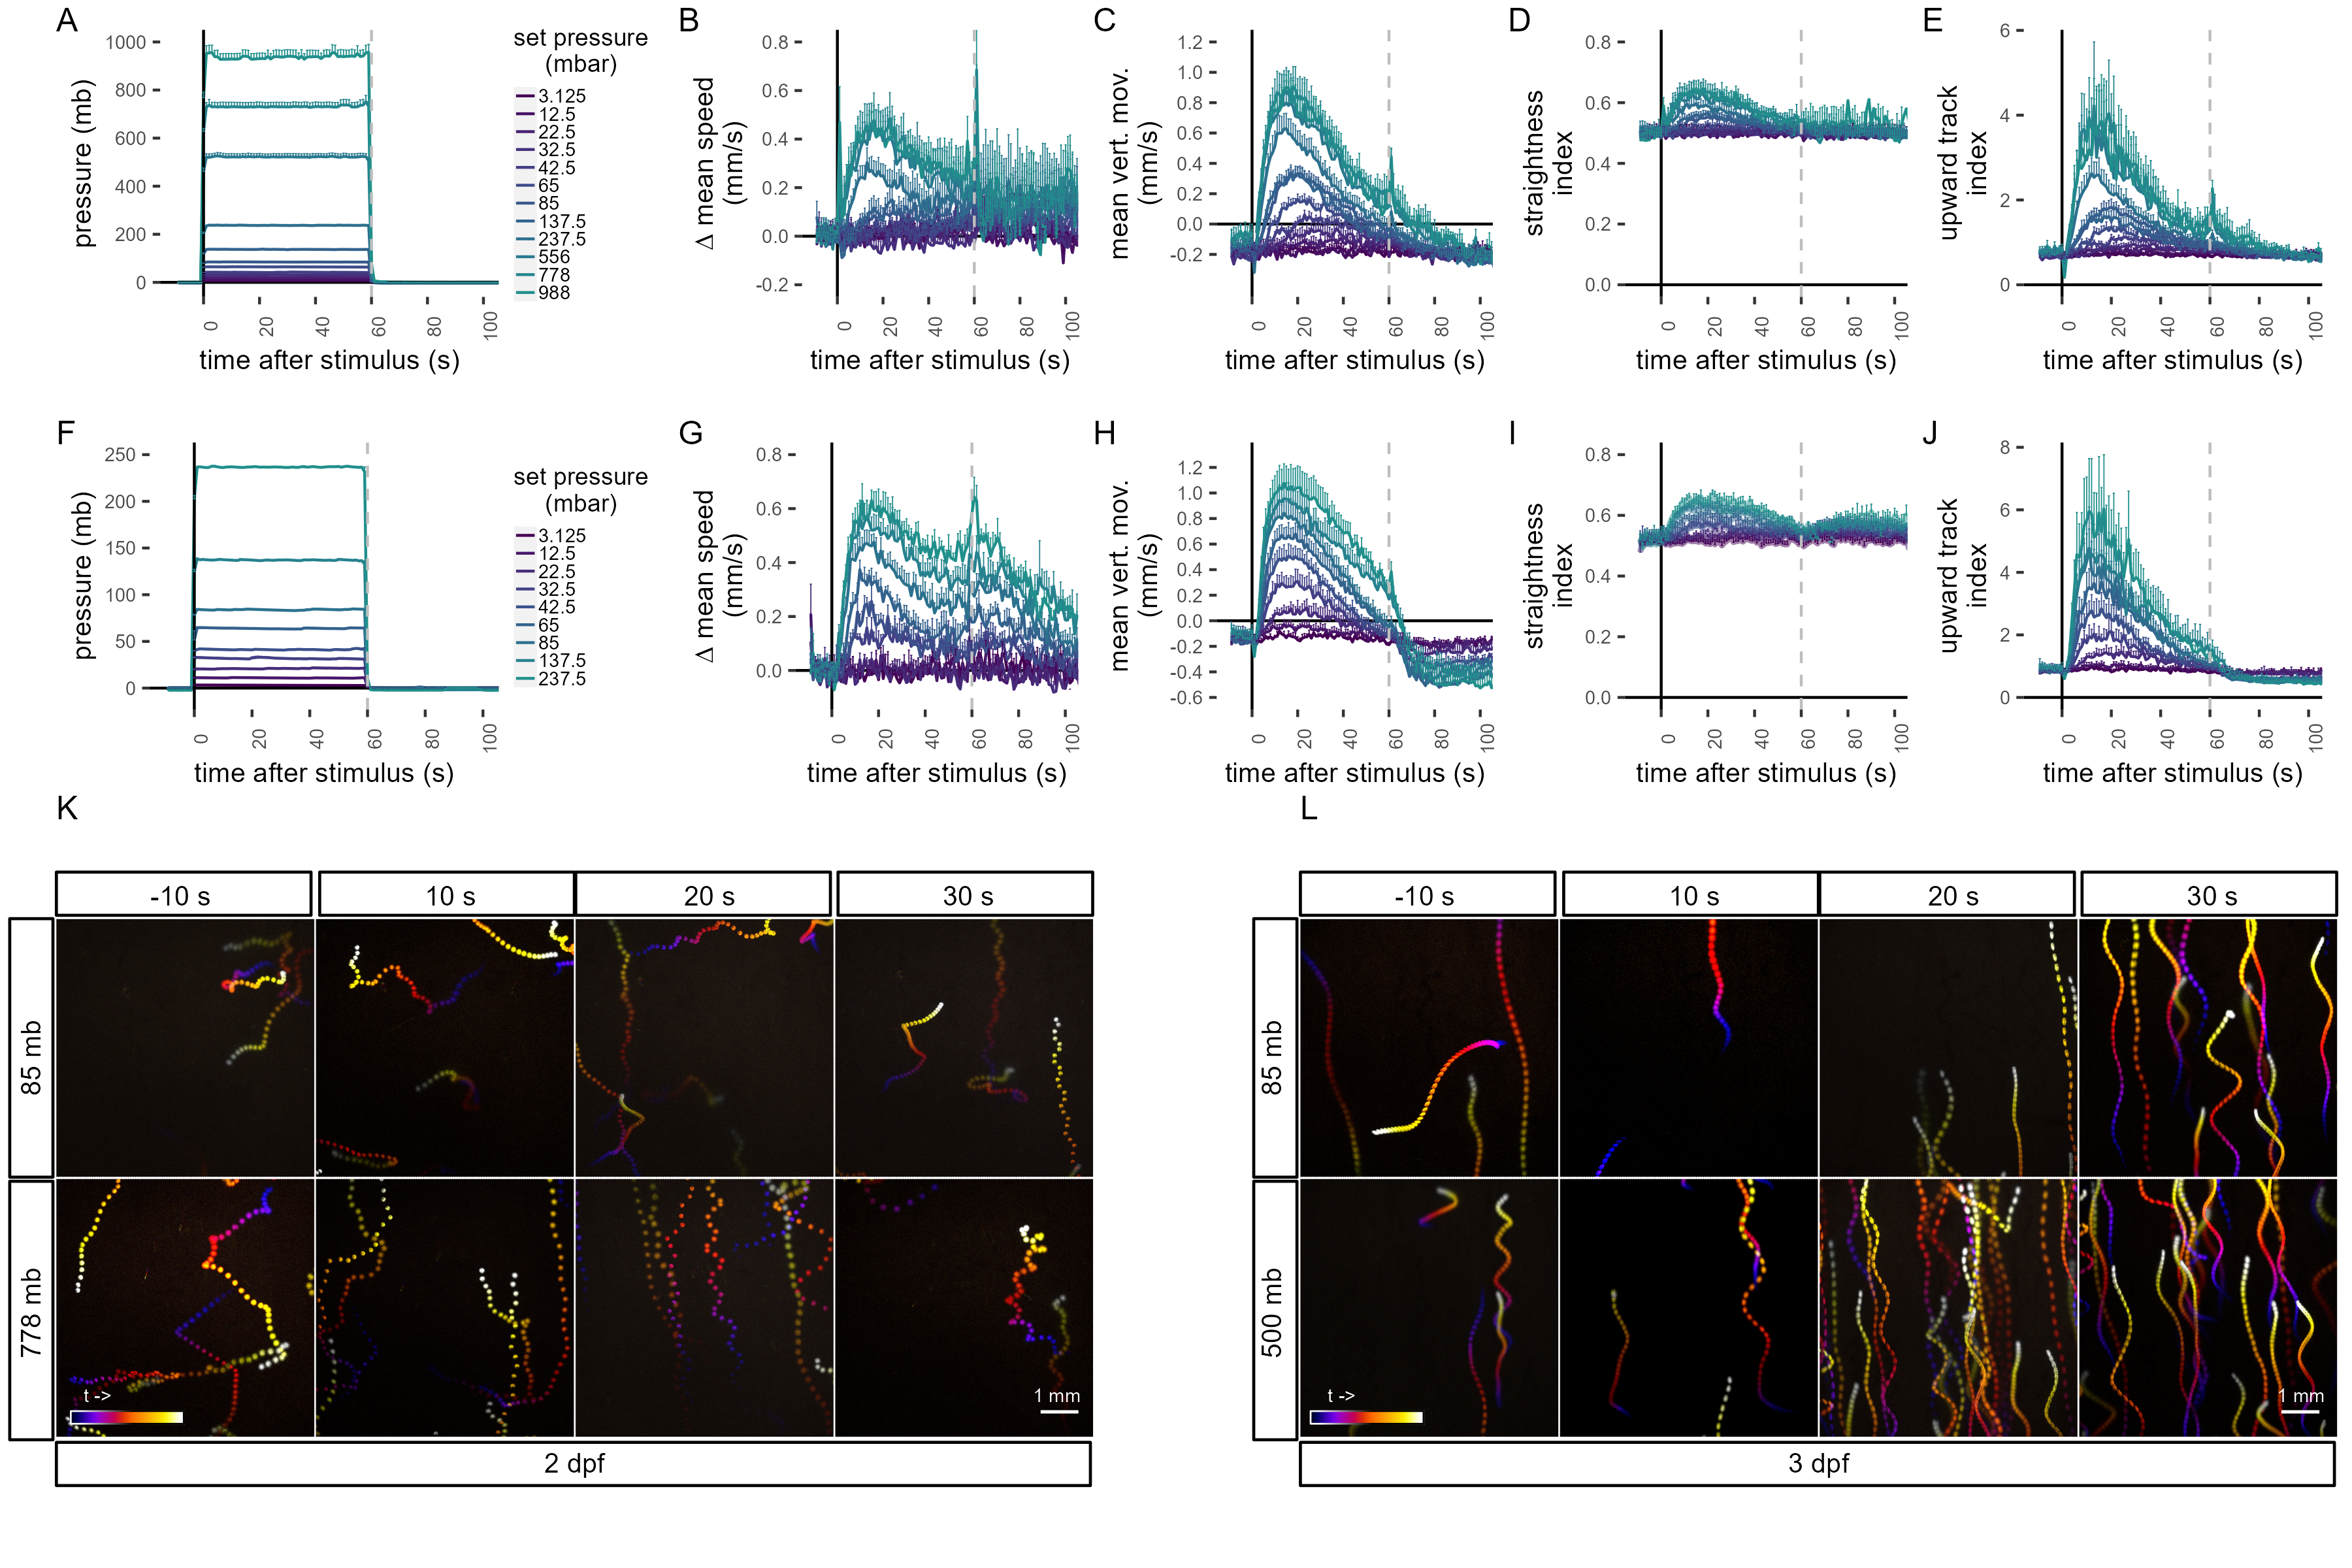
\includegraphics[width=50in]{Figures/Figure1-FigureSupplement1} \caption{**Figure 1—figure supplement 1. ** Quantification of swimming behaviour in *Platynereis* larvae in response to pressure. (A–J) Metrics of the pressure response in two-day-old larvae (A–E), and three-day-old larvae (F–J). Dashed line at 60 s in each plot indicates the end of stimulus. (A,F) Range of step increases in pressure applied to larvae. The step increases were applied in randomized order to each batch of larvae. (B,G) Change in mean speed relative to mean speed before stimulus. (C,H) Mean vertical movement. (D,I) Straightness index. The closer the value is to 1, the less tortuous the track is. (E,J) Upward track index. Defined as the number of upward tracks divided by the number of downward tracks. (K-L) Colour-coded trajectories of 2 day-old (K, Figure 1---Supplement Video 2) and 3 day-old (L, Figure 1---Supplement Video 3) larvae prior and during a step increase in pressure. Trajectories to two different pressure levels are shown, a moderate (top row), and a high (bottom row) step increase. Each projection is 10 seconds long starting 10 s before stimulus (-10 s,left-most column) and ending in the 30 s after stimulus (30 s, right-most column).  Colour code in B–E as in A, and in G–J as in F. Each data point is the average of 2 to 12 (A–E), or 4 to 5 (F–J) batches. Figure 1---source data 1 (A-E), Figure 1---source data 2 (F-J). }\label{fig:unnamed-chunk-7}
\end{figure}

\begin{figure}
\includegraphics[width=36.11in]{Figures/Figure1-FigureSupplement2} \caption{**Figure 1—figure supplement 2. **  (A-B) One-day-old *Platynereis* larvae  do not respond  to small increases in pressure. (A) Range of step increases in pressure applied to one-day-old larvae. (B) Average vertical displacement of one-day-old larvae relative to stimulus onset. Each data point is the average of 1 to 4 batches. (C–E) three-day-old *Platynereis* larvae respond to small changes in hydrostatic pressure applied with a column of water. (C) Schematic of the behavioural setup used to stimulate larvae with a column of water. The height of the column was varied at random between 10 and 200 cm, in 10 cm increments. 1mb ≈ 1cm. (D) Vertical displacement as a function of pressure onset. Vertical dashed line at 20 s indicates end of stimulus. (E) Maximum increase in vertical displacement as a function of pressure. Each data point in D–E is the average of up to 12 batches. Data in B colour-coded as in A. Figure 1---source data 5 (A-B), Figure 1---source data 6 (D-E). }\label{fig:unnamed-chunk-8}
\end{figure}

\begin{figure}
\includegraphics[width=48.61in]{Figures/Figure1-FigureSupplement3} \caption{**Figure 1—figure supplement 3 .** (A–C) Response of three-day-old larvae to a linear increase in pressure.  Each datapoint is the average of 4 to 14 batches. (A) Average linear increase at five different rates (colour code in B) and the fitted curves for the time interval shown. (B) Mean change in vertical displacement at the five different rates of pressure increase shown in A as a function of time. (C) Maximum change in vertical displacement for each rate of pressure increase. Data fitted with either a linear (dashed line) or a 2nd-degree polynomial function (solid line). (D) Average pressure changes applied for data shown in Figure 1F–G. (E–F) Average particle distribution (as a proxy of larval distribution) across the chamber (divided in 5 bins, as schematized in E) prior to pressure stimulus for each batch tested.  (G) Mean change in vertical displacement upon release of pressure from 100 mb and 500 mb after testing the step increases in pressure shown in D. The mean pressure change applied is overlaid on the same plot. (H) Maximum decrease in relative vertical displacement after stimulus start for each set increment in pressure across the 3 acclimation conditions. The "release" dataset consists of the trials shown in G.  Dashed line at 60 s in D and G indicates the point of pressure release and increase, respectively. 5 (0, 100 mb) or 6 (500 mb) batches tested in D—H. Figure 1---source data 7 (A-C), Figure 1---source data 3 (D, F-H).  }\label{fig:unnamed-chunk-9}
\end{figure}

\begin{figure}
\includegraphics[width=34.72in]{Figures/Figure1-FigureSupplement4} \caption{**Figure 1—figure supplement 4. ** Ciliary dynamics assay. (A, top) Schematic of the preparation used to quantify ciliary beat frequency. (A, bottom left) Snapshot of a glued two-day-old larva in the pressure setup. (A, bottom right) Standard deviation projection of time-lapse recording to highlight ciliary band activity. (B) Average pressure levels measured during the experiments corresponding to data shown in Figure 1H. The step increases were applied in randomized order to each larva. (C) Maximum percentage change in CBF during the first 30 s of the stimulus period for each of the step increases in pressure tested. One-tailed unpaired t-test with Bonferroni correction. p-values < 0.05 are shown. Data points from the same larva are joined by lines. N= 18—22 larvae. (D) Individual (thin traces) and mean (thick traces) CBF as a function of pressure level. Dashed line indicates end of pressure stimulus. Figure 1---source data 4 (B-D)}\label{fig:unnamed-chunk-10}
\end{figure}

\begin{figure}
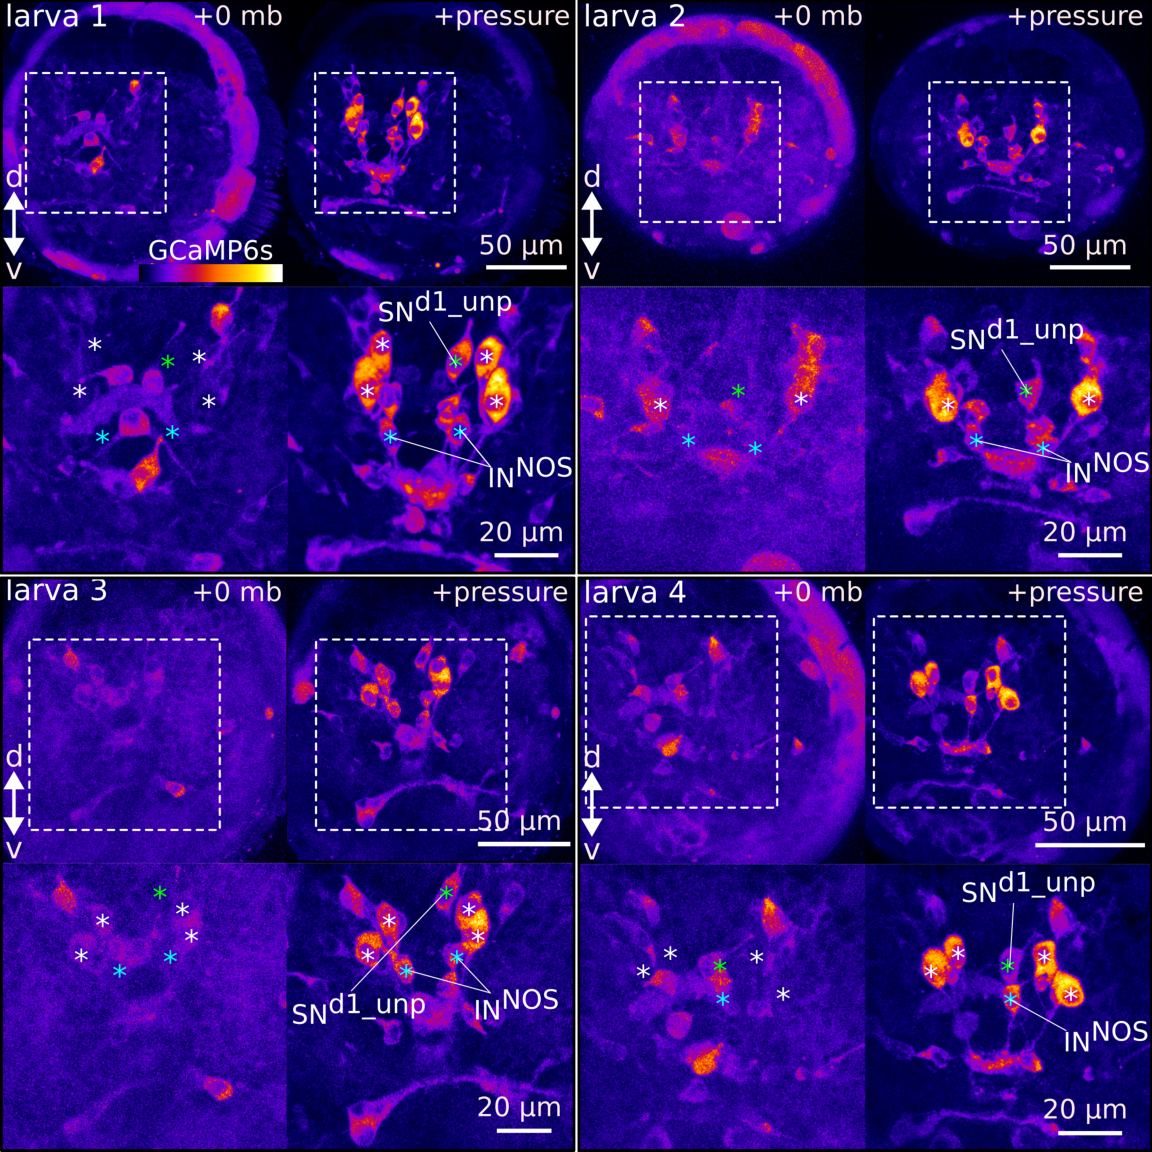
\includegraphics[width=32.01in]{Figures/Figure2-FigureSupplement1} \caption{**Figure 2—figure supplement 1.** Ca²⁺ imaging during pressure increase revealed cells activated during pressure. Maximum intensity projections of two-day-old larvae injected with _GCaMP6s_ mRNA. 4 larvae are shown. (Top panels for each larva) Projections acquired before (+0 mb) or during (+pressure) presentation of the stimulus. (Bottom panels for each larva)  Close-up views of the regions highlighted with dashed squares in the top panels. White asteriks mark the position of cell nuclei of the four sensory cells activated by pressure (cPRCs). Blue asterisk marks the position of the assymetric sensory cell SN^d1_unp^. Green asterisks mark the position of the putative INNOS cells. Pressure > 500 mb in all samples shown.}\label{fig:unnamed-chunk-11}
\end{figure}

\begin{figure}
\includegraphics[width=55.56in]{Figures/Figure2-FigureSupplement2} \caption{**Figure 2—figure supplement 2. ** Ca²⁺ imaging in cPRCs and in SN^d1_unp^. (A) Step pressure increases applied to two-day-old larvae in the Ca²⁺ imaging pressure setup (see Figure 2A). The step increases were applied to each larva in a randomized order. (B) Mean ∆R/R in cPRC_r1, cPRC_l2 and cPRC_r2 as a function of time relative to pressure increase (t = 0). (C) Max.∆R/R in in cPRC_r1, cPRC_l2 and cPRC_r2 as a function of pressure level. One-tailed unpaired t-test with Bonferroni correction testing for an increase in Max.∆R/R with pressure. p-values < 0.05 are shown. (D) ∆R/R in SN^d1_unp^ upon 750 mb pressure increase. Thick line is the mean of individual measuremnts (thinner lines). (E) Individual ∆R/R measurements (thin lines) in the four cPRCs across different steps of pressure increase as a function of time of stimulation. Thicker line is the mean ∆R/R for each pressure level and cell. Dashed lines at 60 s in B-D mark the end of stimulus. N= 2-4 (cPRC_r1),4-5 (cPRC_l2), 4 (cPRC_r2), 4 (SN^d1_unp) cells in B–D. Figure 2---source data 2 (A-E). }\label{fig:unnamed-chunk-12}
\end{figure}

\textbackslash begin\{figure\}
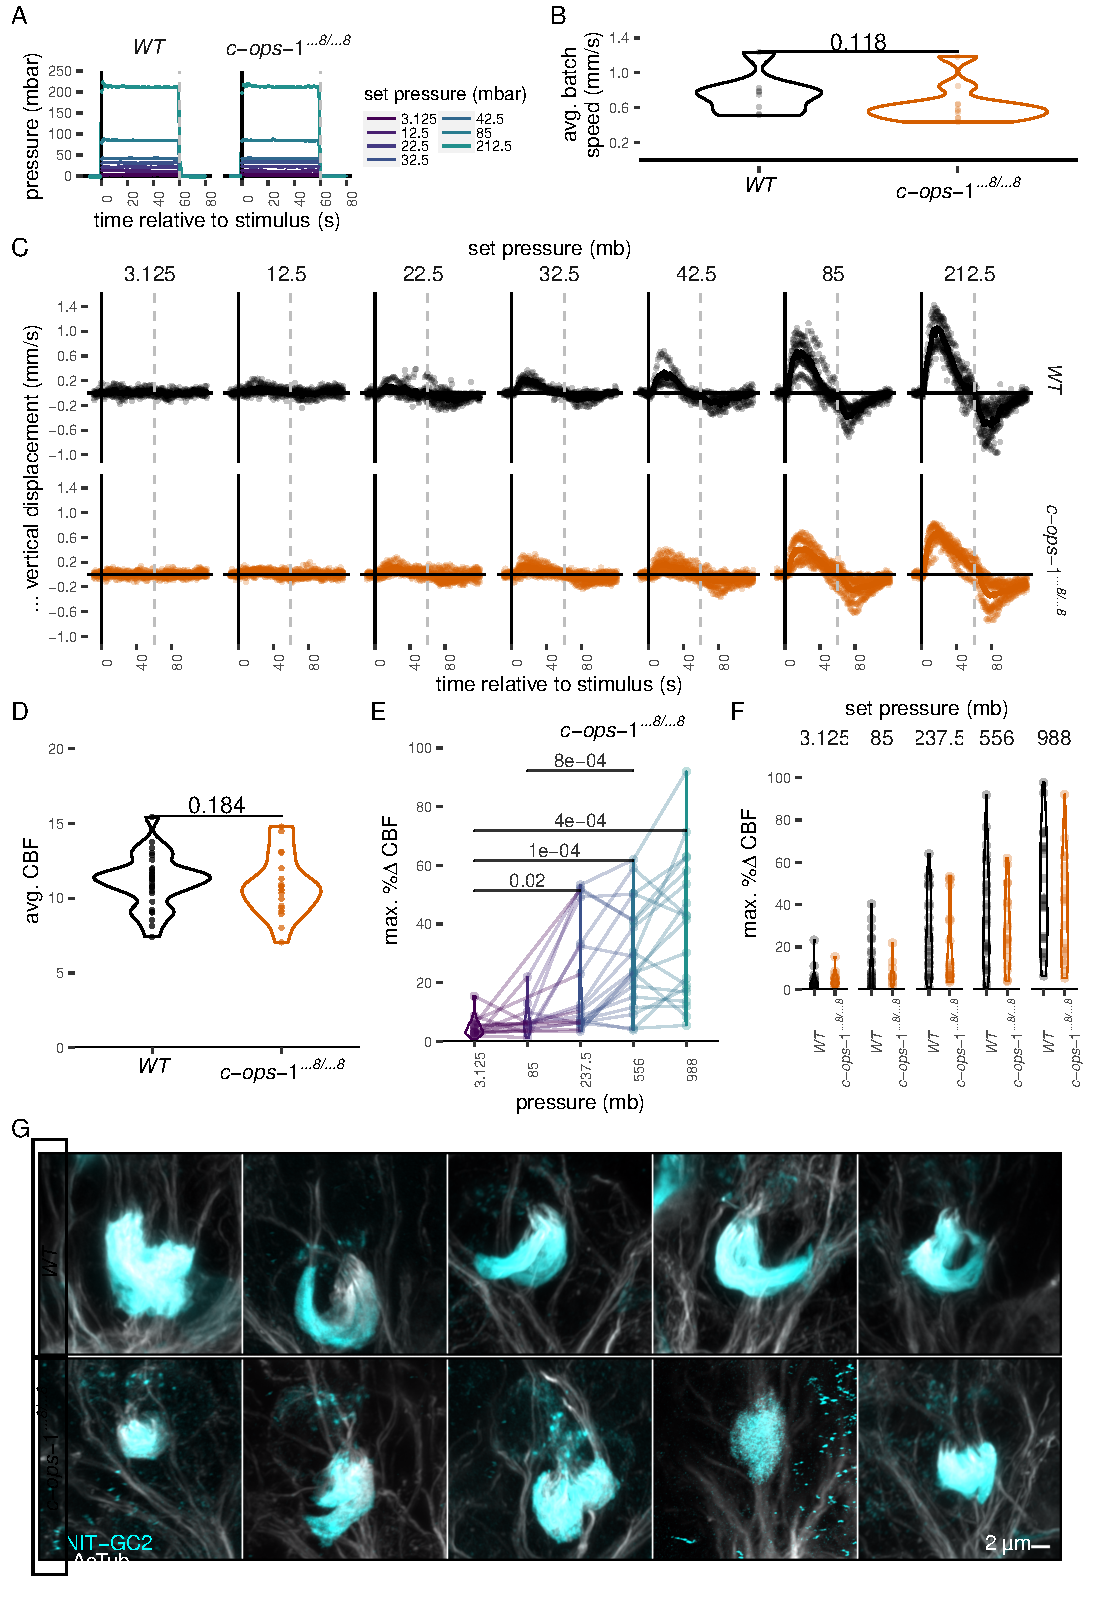
\includegraphics[width=34.72in]{Figures/Figure3-FigureSupplement1}
\textbackslash caption\{\textbf{Figure 3---figure supplement 1. }
Response of three-day-old \emph{c-ops-1\textsuperscript{∆8/∆8}} larvae
to pressure.(A) Mean pressure increase steps applied to three-day-old
\emph{WT} or \emph{c-ops-1\textsuperscript{∆8/∆8}} larvae. (B) Average
swimming speed per batch of \emph{WT} or
\emph{c-ops-1\textsuperscript{∆8/∆8}} larvae in the 10 s prior to
pressure increase. One-tailed unpaired Wilcoxon-test testing for a
decrease in swimming speed in mutant larvae: p = 0.188. (C) Change in
mean vertical displacement as a function of time of stimulation for each
genotype and step increase in pressure. Individual data points are also
plotted. Dashed lines at 60 s mark the end of stimulus. N= 7-9
(\emph{c-ops-1\textsuperscript{∆8/∆8}}) batches, N = 8-10 (\emph{WT})
batches in A---C. (D) Mean CBF for two-day-old \emph{WT} or
\emph{c-ops-1\textsuperscript{∆8/∆8}} larvae in the 30 s prior to
stimulus onset. N = 29 (\emph{WT}) 19
(\emph{c-ops-1\textsuperscript{∆8/∆8}}) larvae. One-tailed unpaired
t-test testing for a decrease in CBF in mutant larvae: p= 0.786. (E)
Maximum \% change in CBF (\% ∆CBF) upon pressure increase in two-day-old
\emph{c-ops-1\textsuperscript{∆8/∆8}} larvae. One-tailed unpaired t-test
with Bonferroni correction. p-values \textless{} 0.05 are shown. N =
10-17 larvae. (F) Maximum percentage change in CBF during the first 30 s
of the stimulus period in WT (N = 18-22 larvae) and in
\emph{c-ops-1\textsuperscript{∆8/∆8}} (N = 10---17 larvae) 2-day-old
larvae. One-tailed unpaired t-test with Bonferroni correction (G) Max.
intensity projections of cPRC cilia of two-day-old \emph{WT} and
\emph{c-ops-1\textsuperscript{∆8/∆8}} larvae used for quantifiying cPRC
ciliary volume (see Figure 3D). Figure 3---source data 1 (A-C), Figure
1---source data 4 (D-F).\}\label{fig:unnamed-chunk-13}
\textbackslash end\{figure\}

\begin{figure}
\includegraphics[width=25.69in]{Figures/Figure3-FigureSupplement2} \caption{**Figure 3—figure supplement 2. ** Morphology of cPRC cilia  in three-day-old _c-ops-1^∆8/∆8^_ larvae. (A) Overview of ultrastucture of cPRC cilia in a _c-ops-1^∆8/∆8^_ larva. Rectangles highlight branches with 2 pairs of microtubule doublets shown in enlarged views on the right. (B) Length of cPRC cilia of _WT_ (N = 15 cilia) and _c-ops-1^∆8/∆8^_ (N = 17 cilia) larvae measured from EM volume reconstructions. Unpaired Wilcoxon test for larger branches in the _WT_ larva: p = 0.228. (C) Length distribution of the branch closest to the basal body (highest Strahler order) for each genotype shown as a percentage of the total ciliary arbor length. One-tailed unpaired Wilcoxon test for longer branches in the mutant: p = 0.082. (E) Ratio of terminal to internal branch lengths of cPRC cilia for each genotype. Unpaired Wilcoxon test for higher terminal-to-internal branch length ratio in the _WT_ larva: p = 0.228. }\label{fig:unnamed-chunk-14}
\end{figure}

\begin{figure}
\includegraphics[width=34.72in]{Figures/Figure4-FigureSupplement1} \caption{**Figure 4—figure supplement 1. ** Effect of TeTxLC-mediated inhibition of serotonergic ciliomotor neurons on CBF during pressure stimulation. (A) Maximum percentage change in CBF during the first 30 s of the stimulus period in 2-day-old larvae injected with the control plasmid TPHp::tdT (N = 14-16 larvae), or with the TPHp::tdT-P2A-TeTxLC plasmid (N = 13-16 larvae).One-tailed unpaired t-test with Bonferroni correction. (B)  Individual (thin traces) and mean (thick traces) CBF as a function of pressure level for larvae injected with the indicated plasmid construct. Dashed line indicates end of pressure stimulus. Figure 4---source data 1 (A-B). }\label{fig:unnamed-chunk-15}
\end{figure}

\hypertarget{references}{%
\section*{References}\label{references}}
\addcontentsline{toc}{section}{References}

\hypertarget{refs}{}
\begin{CSLReferences}{1}{0}
\leavevmode\vadjust pre{\hypertarget{ref-ackermann2005}{}}%
Ackermann, Christian, Adriaan Dorresteijn, and Albrecht Fischer. 2005.
{``Clonal Domains in postlarvalPlatynereis Dumerilii (Annelida:
Polychaeta).''} \emph{Journal of Morphology} 266 (3): 258--80.
\url{https://doi.org/10.1002/jmor.10375}.

\leavevmode\vadjust pre{\hypertarget{ref-akiyama2004}{}}%
Akiyama, Tadashi. 2004. {``Entrainment of the Circatidal Swimming
Activity Rhythm in the Cumacean Dimorphostylis Asiatica (Crustacea) to
12.5-Hour Hydrostatic Pressure Cycles.''} \emph{Zoological Science} 21
(1): 29--38.
\url{https://doi.org/10.2108/0289-0003(2004)21\%5B29:eotcsa\%5D2.0.co;2}.

\leavevmode\vadjust pre{\hypertarget{ref-arendt2004}{}}%
Arendt, Detlev, Kristin Tessmar-Raible, Heidi Snyman, Adriaan W.
Dorresteijn, and Joachim Wittbrodt. 2004. {``Ciliary Photoreceptors with
a Vertebrate-Type Opsin in an Invertebrate Brain.''} \emph{Science} 306
(5697): 869--71. \url{https://doi.org/10.1126/science.1099955}.

\leavevmode\vadjust pre{\hypertarget{ref-baatrup1982}{}}%
Baatrup, Erik. 1982. {``On the Structure of the Corpuscles of de
Quatrefages ({\emph{Branchiostoma Lanceolatum}}(P)).''} \emph{Acta
Zoologica} 63 (1): 39--44.
\url{https://doi.org/10.1111/j.1463-6395.1982.tb00757.x}.

\leavevmode\vadjust pre{\hypertarget{ref-bell2008}{}}%
Bell, Andrew. 2008. {``The Pipe and the Pinwheel: Is Pressure an
Effective Stimulus for the 9+0 Primary Cilium?''} \emph{Cell Biology
International} 32 (4): 462--68.
\url{https://doi.org/10.1016/j.cellbi.2008.03.001}.

\leavevmode\vadjust pre{\hypertarget{ref-bezares-calderon2018}{}}%
Bezares-Calderón, Luis A, Jürgen Berger, Sanja Jasek, Csaba Verasztó,
Sara Mendes, Martin Gühmann, Rodrigo Almeda, Réza Shahidi, and Gáspár
Jékely. 2018. {``Neural Circuitry of a Polycystin-Mediated Hydrodynamic
Startle Response for Predator Avoidance.''} \emph{eLife} 7 (December).
\url{https://doi.org/10.7554/elife.36262}.

\leavevmode\vadjust pre{\hypertarget{ref-bezares-calderon2019}{}}%
Bezares-Calderón, Luis Alberto, Jürgen Berger, and Gáspár Jékely. 2019.
{``Diversity of Cilia-Based Mechanosensory Systems and Their Functions
in Marine Animal Behaviour.''} \emph{Philosophical Transactions of the
Royal Society B: Biological Sciences} 375 (1792): 20190376.
\url{https://doi.org/10.1098/rstb.2019.0376}.

\leavevmode\vadjust pre{\hypertarget{ref-blaxter_1978}{}}%
Blaxter, J. H. S. 1978. {``Baroreception.''} In \emph{Sensory Ecology},
edited by M. A. Ali, 375--409. Boston, {MA}: Springer {US}.
\url{https://doi.org/10.1007/978-1-4684-3363-0/_15}.

\leavevmode\vadjust pre{\hypertarget{ref-bocchero2020}{}}%
Bocchero, Ulisse, Fabio Falleroni, Simone Mortal, Yunzhen Li, Dan Cojoc,
Trevor Lamb, and Vincent Torre. 2020. {``Mechanosensitivity Is an
Essential Component of Phototransduction in Vertebrate Rods.''} Edited
by Samer Hattar. \emph{PLOS Biology} 18 (7): e3000750.
\url{https://doi.org/10.1371/journal.pbio.3000750}.

\leavevmode\vadjust pre{\hypertarget{ref-buxf6hm2016}{}}%
Böhm, Urs Lucas, Andrew Prendergast, Lydia Djenoune, Sophie Nunes
Figueiredo, Johanna Gomez, Caleb Stokes, Sonya Kaiser, et al. 2016.
{``CSF-Contacting Neurons Regulate Locomotion by Relaying Mechanical
Stimuli to Spinal Circuits.''} \emph{Nature Communications} 7 (1).
\url{https://doi.org/10.1038/ncomms10866}.

\leavevmode\vadjust pre{\hypertarget{ref-cardona2012}{}}%
Cardona, Albert, Stephan Saalfeld, Johannes Schindelin, Ignacio
Arganda-Carreras, Stephan Preibisch, Mark Longair, Pavel Tomancak,
Volker Hartenstein, and Rodney J. Douglas. 2012. {``TrakEM2 Software for
Neural Circuit Reconstruction.''} Edited by Aravinthan Samuel.
\emph{PLoS ONE} 7 (6): e38011.
\url{https://doi.org/10.1371/journal.pone.0038011}.

\leavevmode\vadjust pre{\hypertarget{ref-chen2013}{}}%
Chen, Tsai-Wen, Trevor J. Wardill, Yi Sun, Stefan R. Pulver, Sabine L.
Renninger, Amy Baohan, Eric R. Schreiter, et al. 2013. {``Ultrasensitive
Fluorescent Proteins for Imaging Neuronal Activity.''} \emph{Nature} 499
(7458): 295--300. \url{https://doi.org/10.1038/nature12354}.

\leavevmode\vadjust pre{\hypertarget{ref-dynamic2015}{}}%
\emph{Dynamic Documents with r and Knitr, Second Edition}. 2015.
Chapman; Hall/CRC. \url{https://doi.org/10.1201/9781315382487}.

\leavevmode\vadjust pre{\hypertarget{ref-eakin1970}{}}%
Eakin, Richard M., and Aileen Kuda. 1970. {``Ultrastructure of Sensory
Receptors in Ascidian Tadpoles.''} \emph{Zeitschrift Für Zellforschung
Und Mikroskopische Anatomie} 112 (3): 287--312.
\url{https://doi.org/10.1007/bf02584045}.

\leavevmode\vadjust pre{\hypertarget{ref-edelstein2010}{}}%
Edelstein, Arthur, Nenad Amodaj, Karl Hoover, Ron Vale, and Nico
Stuurman. 2010. {``Computer Control of Microscopes Using µManager.''}
\emph{Current Protocols in Molecular Biology} 92 (1).
\url{https://doi.org/10.1002/0471142727.mb1420s92}.

\leavevmode\vadjust pre{\hypertarget{ref-fernandez2020}{}}%
Fernandez, Romain, and Cédric Moisy. 2020. {``Fijiyama: A Registration
Tool for 3D Multimodal Time-Lapse Imaging.''} Edited by Xu Jinbo.
\emph{Bioinformatics} 37 (10): 1482--84.
\url{https://doi.org/10.1093/bioinformatics/btaa846}.

\leavevmode\vadjust pre{\hypertarget{ref-fischer2010}{}}%
Fischer, Antje HL, Thorsten Henrich, and Detlev Arendt. 2010. {``The
Normal Development of Platynereis Dumerilii (Nereididae, Annelida).''}
\emph{Frontiers in Zoology} 7 (1): 31.
\url{https://doi.org/10.1186/1742-9994-7-31}.

\leavevmode\vadjust pre{\hypertarget{ref-forward_1989c}{}}%
Forward, RB, CA Wellins, and CU Buswell. 1989. {``Behavioral Responses
of Larvae of the Crab Neopanope Sayi to Hydrostatic Pressure.''}
\emph{Marine Ecology Progress Series} 57: 267--77.
\url{https://doi.org/10.3354/meps057267}.

\leavevmode\vadjust pre{\hypertarget{ref-fraser_1994}{}}%
Fraser, Peter J., and Alister G. Macdonald. 1994. {``Crab Hydrostatic
Pressure Sensors.''} \emph{Nature} 371 (6496): 383--84.
\url{https://doi.org/10.1038/371383b0}.

\leavevmode\vadjust pre{\hypertarget{ref-fraser_2002}{}}%
Fraser, Peter J, and Richard L Shelmerdine. 2002. {``Dogfish Hair Cells
Sense Hydrostatic Pressure.''} \emph{Nature} 415 (6871): 495--96.
\url{https://doi.org/10.1038/415495a}.

\leavevmode\vadjust pre{\hypertarget{ref-gambi1992}{}}%
Gambi, Maria Cristina, Maurizio Lorenti, Giovanni F. Russo, Maria
Beatrice Scipione, and Valerio Zupo. 1992. {``Depth and Seasonal
Distribution of Some Groups of the Vagile Fauna of the Posidonia
Oceanica Leaf Stratum: Structural and Trophic Analyses.''} \emph{Marine
Ecology} 13 (1): 17--39.
\url{https://doi.org/10.1111/j.1439-0485.1992.tb00337.x}.

\leavevmode\vadjust pre{\hypertarget{ref-genin2005a}{}}%
Genin, Amatzia, Jules S. Jaffe, Ruth Reef, Claudio Richter, and Peter J.
S. Franks. 2005. {``Swimming Against the Flow: A Mechanism of
Zooplankton Aggregation.''} \emph{Science} 308 (5723): 860--62.
\url{https://doi.org/10.1126/science.1107834}.

\leavevmode\vadjust pre{\hypertarget{ref-ghmann_2015}{}}%
Gühmann, Martin, Huiyong Jia, Nadine Randel, Csaba Verasztó, Luis A
Bezares-Calderón, Nico K Michiels, Shozo Yokoyama, and Gáspár Jékely.
2015. {``Spectral Tuning of Phototaxis by a Go-Opsin in the Rhabdomeric
Eyes of Platynereis.''} \emph{Current Biology} 25 (17): 2265--71.
\url{https://doi.org/10.1016/j.cub.2015.07.017}.

\leavevmode\vadjust pre{\hypertarget{ref-hernandez-nicaise1984}{}}%
Hernandez-Nicaise, Mari-Luz. 1984. {``Ctenophora.''} In, 96--111.
Springer Berlin Heidelberg.
\url{https://doi.org/10.1007/978-3-642-51593-4_9}.

\leavevmode\vadjust pre{\hypertarget{ref-iatsenko2016}{}}%
Iatsenko, D., P. V. E. McClintock, and A. Stefanovska. 2016.
{``Extraction of Instantaneous Frequencies from Ridges in
Time{\textendash}frequency Representations of Signals.''} \emph{Signal
Processing} 125 (August): 290--303.
\url{https://doi.org/10.1016/j.sigpro.2016.01.024}.

\leavevmode\vadjust pre{\hypertarget{ref-iatsenko2019}{}}%
Iatsenko, Dmytro, Gemma Lancaster, Sam McCormack, Julian Newman, Guru
Vamsi Policharla, Valentina Ticcinelli, Tomislav Stankovski, and Aneta
Stefanovska. 2019. \emph{MODA V1.01}. Zenodo.
\url{https://doi.org/10.5281/ZENODO.3470856}.

\leavevmode\vadjust pre{\hypertarget{ref-imambocus2022}{}}%
Imambocus, Bibi Nusreen, Fangmin Zhou, Andrey Formozov, Annika Wittich,
Federico M. Tenedini, Chun Hu, Kathrin Sauter, et al. 2022. {``A
Neuropeptidergic Circuit Gates Selective Escape Behavior of Drosophila
Larvae.''} \emph{Current Biology} 32 (1): 149--163.e8.
\url{https://doi.org/10.1016/j.cub.2021.10.069}.

\leavevmode\vadjust pre{\hypertarget{ref-jasek2022}{}}%
Jasek, Sanja, Csaba Verasztó, Emelie Brodrick, Réza Shahidi, Tom
Kazimiers, Alexandra Kerbl, and Gáspár Jékely. 2022. {``Desmosomal
Connectomics of All Somatic Muscles in an Annelid Larva.''} \emph{eLife}
11 (December). \url{https://doi.org/10.7554/elife.71231}.

\leavevmode\vadjust pre{\hypertarget{ref-jokura2023}{}}%
Jokura, Kei, Nobuo Ueda, Martin Gühmann, Luis Alfonso Yañez-Guerra,
Piotr Słowiński, Kyle C. A. Wedgwood, and Gáspár Jékely. 2023. {``Nitric
Oxide Feedback to Ciliary Photoreceptor Cells Gates a UV Avoidance
Circuit.''} \url{http://dx.doi.org/10.1101/2023.08.02.551600}.

\leavevmode\vadjust pre{\hypertarget{ref-knightjones_1955}{}}%
Knight-Jones, E W, and S Z Qasim. 1955. {``Responses of Some Marine
Plankton Animals to Changes in Hydrostatic Pressure.''} \emph{Nature}
175 (4465): 941--42. \url{https://www.ncbi.nlm.nih.gov/pubmed/14383773}.

\leavevmode\vadjust pre{\hypertarget{ref-lem1999}{}}%
Lem, J., N. V. Krasnoperova, P. D. Calvert, B. Kosaras, D. A. Cameron,
M. Nicolò, C. L. Makino, and R. L. Sidman. 1999. {``Morphological,
Physiological, and Biochemical Changes in Rhodopsin Knockout Mice.''}
\emph{Proceedings of the National Academy of Sciences} 96 (2): 736--41.
\url{https://doi.org/10.1073/pnas.96.2.736}.

\leavevmode\vadjust pre{\hypertarget{ref-li2022a}{}}%
Li, Yuhui, Ondřej Kučera, Damien Cuvelier, David M. Rutkowski, Mathieu
Deygas, Dipti Rai, Tonja Pavlovič, et al. 2022. {``Compressive Forces
Stabilise Microtubules in Living Cells.''}
\url{http://dx.doi.org/10.1101/2022.02.07.479347}.

\leavevmode\vadjust pre{\hypertarget{ref-lincoln_1970}{}}%
Lincoln, R. J., and I. Gilchrist. 1970. {``An Observational Pressure
Vessel for Studying the Behaviour of Planktonic Animals.''} \emph{Marine
Biology} 6 (1): 1--4. \url{https://doi.org/10.1007/\%7BBF00352600\%7D}.

\leavevmode\vadjust pre{\hypertarget{ref-liu2015}{}}%
Liu, Chao, and Craig Montell. 2015. {``Forcing Open TRP Channels:
Mechanical Gating as a Unifying Activation Mechanism.''}
\emph{Biochemical and Biophysical Research Communications} 460 (1):
22--25. \url{https://doi.org/10.1016/j.bbrc.2015.02.067}.

\leavevmode\vadjust pre{\hypertarget{ref-luo2014}{}}%
Luo, Na, Michael D. Conwell, Xingjuan Chen, Christine Insinna
Kettenhofen, Christopher J. Westlake, Louis B. Cantor, Clark D. Wells,
et al. 2014. {``Primary Cilia Signaling Mediates Intraocular Pressure
Sensation.''} \emph{Proceedings of the National Academy of Sciences} 111
(35): 12871--76. \url{https://doi.org/10.1073/pnas.1323292111}.

\leavevmode\vadjust pre{\hypertarget{ref-mcdonald2011}{}}%
McDONALD, K. L., and R. I. WEBB. 2011. {``Freeze Substitution in 3 Hours
or Less.''} \emph{Journal of Microscopy} 243 (3): 227--33.
\url{https://doi.org/10.1111/j.1365-2818.2011.03526.x}.

\leavevmode\vadjust pre{\hypertarget{ref-morgan1965}{}}%
Morgan, Elfed. 1965. {``The Activity Rhythm of the Amphipod Corophium
Volutator (Pallas) and Its Possible Relationship to Changes in
Hydrostatic Pressure Associated with the Tides.''} \emph{The Journal of
Animal Ecology} 34 (3): 731. \url{https://doi.org/10.2307/2459}.

\leavevmode\vadjust pre{\hypertarget{ref-morgan_1984}{}}%
---------. 1984. {``The Pressure-Responses of Marine Invertebrates: A
Psychophysical Perspective.''} \emph{Zoological Journal of the Linnean
Society} 80 (2-3): 209--30.
\url{https://doi.org/10.1111/j.1096-3642.1984.tb01974.x}.

\leavevmode\vadjust pre{\hypertarget{ref-nasrin2021}{}}%
Nasrin, Syeda Rubaiya, Christian Ganser, Seiji Nishikawa, Arif Md.
Rashedul Kabir, Kazuki Sada, Takefumi Yamashita, Mitsunori Ikeguchi,
Takayuki Uchihashi, Henry Hess, and Akira Kakugo. 2021. {``Deformation
of Microtubules Regulates Translocation Dynamics of Kinesin.''}
\emph{Science Advances} 7 (42).
\url{https://doi.org/10.1126/sciadv.abf2211}.

\leavevmode\vadjust pre{\hypertarget{ref-naylor1984a}{}}%
Naylor, E., and Barbara G. Williams. 1984. {``Phase-Responsiveness of
the Circatidal Locomotor Activity Rhythm of {\emph{Hemigrapsus
Edwardsi}} (Hilgendorf) to Simulated High Tide.''} \emph{Journal of the
Marine Biological Association of the United Kingdom} 64 (1): 81--90.
\url{https://doi.org/10.1017/s0025315400059646}.

\leavevmode\vadjust pre{\hypertarget{ref-uxf6zpolat2021}{}}%
Özpolat, B. Duygu, Nadine Randel, Elizabeth A. Williams, Luis Alberto
Bezares-Calderón, Gabriele Andreatta, Guillaume Balavoine, Paola Y.
Bertucci, et al. 2021. {``The Nereid on the Rise: Platynereis as a Model
System.''} \emph{EvoDevo} 12 (1).
\url{https://doi.org/10.1186/s13227-021-00180-3}.

\leavevmode\vadjust pre{\hypertarget{ref-pang2021}{}}%
Pang, Ji-Jie, Fan Gao, and Samuel M. Wu. 2021. {``Generators of
Pressure-Evoked Currents in Vertebrate Outer Retinal Neurons.''}
\emph{Cells} 10 (6): 1288. \url{https://doi.org/10.3390/cells10061288}.

\leavevmode\vadjust pre{\hypertarget{ref-pattappa2019}{}}%
Pattappa, G, J Zellner, B Johnstone, D Docheva, and P Angele. 2019.
{``Cells Under Pressure {\textendash} the Relationship Between
Hydrostatic Pressure and Mesenchymal Stem Cell Chondrogenesis.''}
\emph{European Cells and Materials} 36 (May): 360--81.
\url{https://doi.org/10.22203/ecm.v037a22}.

\leavevmode\vadjust pre{\hypertarget{ref-preibisch2010}{}}%
Preibisch, Stephan, Stephan Saalfeld, Johannes Schindelin, and Pavel
Tomancak. 2010. {``Software for Bead-Based Registration of Selective
Plane Illumination Microscopy Data.''} \emph{Nature Methods} 7 (6):
418--19. \url{https://doi.org/10.1038/nmeth0610-418}.

\leavevmode\vadjust pre{\hypertarget{ref-qutob1963}{}}%
Qutob, Ziad. 1963. {``The Swimbladder of Fishes as a Pressure
Receptor.''} \emph{Archives Néerlandaises de Zoologie} 15 (1): 1--67.
\url{https://doi.org/10.1163/036551662x00015}.

\leavevmode\vadjust pre{\hypertarget{ref-ferreira2019}{}}%
R. Ferreira, Rita, Hajime Fukui, Renee Chow, Andrej Vilfan, and Julien
Vermot. 2019. {``The Cilium as a Force Sensor{-}Myth Versus Reality.''}
\emph{Journal of Cell Science} 132 (14).
\url{https://doi.org/10.1242/jcs.213496}.

\leavevmode\vadjust pre{\hypertarget{ref-randel2014}{}}%
Randel, Nadine, Albina Asadulina, Luis A Bezares-Calderón, Csaba
Verasztó, Elizabeth A Williams, Markus Conzelmann, Réza Shahidi, and
Gáspár Jékely. 2014. {``Neuronal Connectome of a Sensory-Motor Circuit
for Visual Navigation.''} \emph{eLife} 3 (May).
\url{https://doi.org/10.7554/elife.02730}.

\leavevmode\vadjust pre{\hypertarget{ref-rice_1964}{}}%
Rice, A. L. 1964. {``Observations on the Effects of Changes of
Hydrostatic Pressure on the Behaviour of Some Marine Animals.''}
\emph{Journal of the Marine Biological Association of the {UK}} 44 (01):
163. \url{https://doi.org/10.1017/S0025315400024723}.

\leavevmode\vadjust pre{\hypertarget{ref-saalfeld2009}{}}%
Saalfeld, Stephan, Albert Cardona, Volker Hartenstein, and Pavel
Tomančák. 2009. {``CATMAID: Collaborative Annotation Toolkit for Massive
Amounts of Image Data.''} \emph{Bioinformatics} 25 (15): 1984--86.
\url{https://doi.org/10.1093/bioinformatics/btp266}.

\leavevmode\vadjust pre{\hypertarget{ref-sulkin_1984}{}}%
Sulkin, SD. 1984. {``Behavioral Basis of Depth Regulation in the Larvae
of Brachyuran Crabs.''} \emph{Marine Ecology Progress Series} 15:
181--205. \url{https://doi.org/10.3354/meps015181}.

\leavevmode\vadjust pre{\hypertarget{ref-sweeney1995}{}}%
Sweeney, Sean T, Kendal Broadie, John Keane, Heiner Niemann, and Cahir J
O'Kane. 1995. {``Targeted Expression of Tetanus Toxin Light Chain in
Drosophila Specifically Eliminates Synaptic Transmission and Causes
Behavioral Defects.''} \emph{Neuron} 14 (2): 341--51.
\url{https://doi.org/10.1016/0896-6273(95)90290-2}.

\leavevmode\vadjust pre{\hypertarget{ref-tessmar-raible2007}{}}%
Tessmar-Raible, Kristin, Florian Raible, Foteini Christodoulou, Keren
Guy, Martina Rembold, Harald Hausen, and Detlev Arendt. 2007.
{``Conserved Sensory-Neurosecretory Cell Types in Annelid and Fish
Forebrain: Insights into Hypothalamus Evolution.''} \emph{Cell} 129 (7):
1389--1400. \url{https://doi.org/10.1016/j.cell.2007.04.041}.

\leavevmode\vadjust pre{\hypertarget{ref-tosches2014}{}}%
Tosches, Maria~Antonietta, Daniel Bucher, Pavel Vopalensky, and Detlev
Arendt. 2014. {``Melatonin Signaling Controls Circadian Swimming
Behavior in Marine Zooplankton.''} \emph{Cell} 159 (1): 46--57.
\url{https://doi.org/10.1016/j.cell.2014.07.042}.

\leavevmode\vadjust pre{\hypertarget{ref-Tsukamoto2017}{}}%
Tsukamoto, Hisao, I-Shan Chen, Yoshihiro Kubo, and Yuji Furutani. 2017.
{``A Ciliary Opsin in the Brain of a Marine Annelid Zooplankton Is
Ultraviolet-Sensitive, and the Sensitivity Is Tuned by a Single Amino
Acid Residue.''} \emph{Journal of Biological Chemistry} 292 (31):
12971--80. \url{https://doi.org/10.1074/jbc.m117.793539}.

\leavevmode\vadjust pre{\hypertarget{ref-veraszto2018}{}}%
Verasztó, Csaba, Martin Gühmann, Huiyong Jia, Vinoth Babu Veedin Rajan,
Luis A Bezares-Calderón, Cristina Piñeiro-Lopez, Nadine Randel, et al.
2018. {``Ciliary and Rhabdomeric Photoreceptor-Cell Circuits Form a
Spectral Depth Gauge in Marine Zooplankton.''} \emph{eLife} 7 (May).
\url{https://doi.org/10.7554/elife.36440}.

\leavevmode\vadjust pre{\hypertarget{ref-veraszto2020}{}}%
Verasztó, Csaba, Sanja Jasek, Martin Gühmann, Réza Shahidi, Nobuo Ueda,
James David Beard, Sara Mendes, et al. 2020. {``Whole-Animal Connectome
and Cell-Type Complement of the Three-Segmented {\emph{Platynereis
Dumerilii}} Larva.''} \url{http://dx.doi.org/10.1101/2020.08.21.260984}.

\leavevmode\vadjust pre{\hypertarget{ref-veraszto2017a}{}}%
Verasztó, Csaba, Nobuo Ueda, Luis A Bezares-Calderón, Aurora Panzera,
Elizabeth A Williams, Réza Shahidi, and Gáspár Jékely. 2017.
{``Ciliomotor Circuitry Underlying Whole-Body Coordination of Ciliary
Activity in the Platynereis Larva.''} \emph{eLife} 6 (May).
\url{https://doi.org/10.7554/elife.26000}.

\leavevmode\vadjust pre{\hypertarget{ref-williams2017}{}}%
Williams, Elizabeth A, Csaba Verasztó, Sanja Jasek, Markus Conzelmann,
Réza Shahidi, Philipp Bauknecht, Olivier Mirabeau, and Gáspár Jékely.
2017. {``Synaptic and Peptidergic Connectome of a Neurosecretory Center
in the Annelid Brain.''} \emph{eLife} 6 (December).
\url{https://doi.org/10.7554/elife.26349}.

\leavevmode\vadjust pre{\hypertarget{ref-zanini2018}{}}%
Zanini, Damiano, Diego Giraldo, Ben Warren, Radoslaw Katana, Marta
Andrés, Suneel Reddy, Stephanie Pauls, Nicola Schwedhelm-Domeyer, Bart
R. H. Geurten, and Martin C. Göpfert. 2018. {``Proprioceptive Opsin
Functions in Drosophila Larval Locomotion.''} \emph{Neuron} 98 (1):
67--74.e4. \url{https://doi.org/10.1016/j.neuron.2018.02.028}.

\end{CSLReferences}

\end{document}
